% Options for packages loaded elsewhere
\PassOptionsToPackage{unicode}{hyperref}
\PassOptionsToPackage{hyphens}{url}
%
\documentclass[
]{book}
\usepackage{amsmath,amssymb}
\usepackage{iftex}
\ifPDFTeX
  \usepackage[T1]{fontenc}
  \usepackage[utf8]{inputenc}
  \usepackage{textcomp} % provide euro and other symbols
\else % if luatex or xetex
  \usepackage{unicode-math} % this also loads fontspec
  \defaultfontfeatures{Scale=MatchLowercase}
  \defaultfontfeatures[\rmfamily]{Ligatures=TeX,Scale=1}
\fi
\usepackage{lmodern}
\ifPDFTeX\else
  % xetex/luatex font selection
\fi
% Use upquote if available, for straight quotes in verbatim environments
\IfFileExists{upquote.sty}{\usepackage{upquote}}{}
\IfFileExists{microtype.sty}{% use microtype if available
  \usepackage[]{microtype}
  \UseMicrotypeSet[protrusion]{basicmath} % disable protrusion for tt fonts
}{}
\makeatletter
\@ifundefined{KOMAClassName}{% if non-KOMA class
  \IfFileExists{parskip.sty}{%
    \usepackage{parskip}
  }{% else
    \setlength{\parindent}{0pt}
    \setlength{\parskip}{6pt plus 2pt minus 1pt}}
}{% if KOMA class
  \KOMAoptions{parskip=half}}
\makeatother
\usepackage{xcolor}
\usepackage{color}
\usepackage{fancyvrb}
\newcommand{\VerbBar}{|}
\newcommand{\VERB}{\Verb[commandchars=\\\{\}]}
\DefineVerbatimEnvironment{Highlighting}{Verbatim}{commandchars=\\\{\}}
% Add ',fontsize=\small' for more characters per line
\usepackage{framed}
\definecolor{shadecolor}{RGB}{248,248,248}
\newenvironment{Shaded}{\begin{snugshade}}{\end{snugshade}}
\newcommand{\AlertTok}[1]{\textcolor[rgb]{0.94,0.16,0.16}{#1}}
\newcommand{\AnnotationTok}[1]{\textcolor[rgb]{0.56,0.35,0.01}{\textbf{\textit{#1}}}}
\newcommand{\AttributeTok}[1]{\textcolor[rgb]{0.13,0.29,0.53}{#1}}
\newcommand{\BaseNTok}[1]{\textcolor[rgb]{0.00,0.00,0.81}{#1}}
\newcommand{\BuiltInTok}[1]{#1}
\newcommand{\CharTok}[1]{\textcolor[rgb]{0.31,0.60,0.02}{#1}}
\newcommand{\CommentTok}[1]{\textcolor[rgb]{0.56,0.35,0.01}{\textit{#1}}}
\newcommand{\CommentVarTok}[1]{\textcolor[rgb]{0.56,0.35,0.01}{\textbf{\textit{#1}}}}
\newcommand{\ConstantTok}[1]{\textcolor[rgb]{0.56,0.35,0.01}{#1}}
\newcommand{\ControlFlowTok}[1]{\textcolor[rgb]{0.13,0.29,0.53}{\textbf{#1}}}
\newcommand{\DataTypeTok}[1]{\textcolor[rgb]{0.13,0.29,0.53}{#1}}
\newcommand{\DecValTok}[1]{\textcolor[rgb]{0.00,0.00,0.81}{#1}}
\newcommand{\DocumentationTok}[1]{\textcolor[rgb]{0.56,0.35,0.01}{\textbf{\textit{#1}}}}
\newcommand{\ErrorTok}[1]{\textcolor[rgb]{0.64,0.00,0.00}{\textbf{#1}}}
\newcommand{\ExtensionTok}[1]{#1}
\newcommand{\FloatTok}[1]{\textcolor[rgb]{0.00,0.00,0.81}{#1}}
\newcommand{\FunctionTok}[1]{\textcolor[rgb]{0.13,0.29,0.53}{\textbf{#1}}}
\newcommand{\ImportTok}[1]{#1}
\newcommand{\InformationTok}[1]{\textcolor[rgb]{0.56,0.35,0.01}{\textbf{\textit{#1}}}}
\newcommand{\KeywordTok}[1]{\textcolor[rgb]{0.13,0.29,0.53}{\textbf{#1}}}
\newcommand{\NormalTok}[1]{#1}
\newcommand{\OperatorTok}[1]{\textcolor[rgb]{0.81,0.36,0.00}{\textbf{#1}}}
\newcommand{\OtherTok}[1]{\textcolor[rgb]{0.56,0.35,0.01}{#1}}
\newcommand{\PreprocessorTok}[1]{\textcolor[rgb]{0.56,0.35,0.01}{\textit{#1}}}
\newcommand{\RegionMarkerTok}[1]{#1}
\newcommand{\SpecialCharTok}[1]{\textcolor[rgb]{0.81,0.36,0.00}{\textbf{#1}}}
\newcommand{\SpecialStringTok}[1]{\textcolor[rgb]{0.31,0.60,0.02}{#1}}
\newcommand{\StringTok}[1]{\textcolor[rgb]{0.31,0.60,0.02}{#1}}
\newcommand{\VariableTok}[1]{\textcolor[rgb]{0.00,0.00,0.00}{#1}}
\newcommand{\VerbatimStringTok}[1]{\textcolor[rgb]{0.31,0.60,0.02}{#1}}
\newcommand{\WarningTok}[1]{\textcolor[rgb]{0.56,0.35,0.01}{\textbf{\textit{#1}}}}
\usepackage{longtable,booktabs,array}
\usepackage{calc} % for calculating minipage widths
% Correct order of tables after \paragraph or \subparagraph
\usepackage{etoolbox}
\makeatletter
\patchcmd\longtable{\par}{\if@noskipsec\mbox{}\fi\par}{}{}
\makeatother
% Allow footnotes in longtable head/foot
\IfFileExists{footnotehyper.sty}{\usepackage{footnotehyper}}{\usepackage{footnote}}
\makesavenoteenv{longtable}
\usepackage{graphicx}
\makeatletter
\def\maxwidth{\ifdim\Gin@nat@width>\linewidth\linewidth\else\Gin@nat@width\fi}
\def\maxheight{\ifdim\Gin@nat@height>\textheight\textheight\else\Gin@nat@height\fi}
\makeatother
% Scale images if necessary, so that they will not overflow the page
% margins by default, and it is still possible to overwrite the defaults
% using explicit options in \includegraphics[width, height, ...]{}
\setkeys{Gin}{width=\maxwidth,height=\maxheight,keepaspectratio}
% Set default figure placement to htbp
\makeatletter
\def\fps@figure{htbp}
\makeatother
\setlength{\emergencystretch}{3em} % prevent overfull lines
\providecommand{\tightlist}{%
  \setlength{\itemsep}{0pt}\setlength{\parskip}{0pt}}
\setcounter{secnumdepth}{5}
\usepackage{booktabs}
\ifLuaTeX
  \usepackage{selnolig}  % disable illegal ligatures
\fi
\usepackage[]{natbib}
\bibliographystyle{plainnat}
\IfFileExists{bookmark.sty}{\usepackage{bookmark}}{\usepackage{hyperref}}
\IfFileExists{xurl.sty}{\usepackage{xurl}}{} % add URL line breaks if available
\urlstyle{same}
\hypersetup{
  pdftitle={Introducción al software R},
  pdfauthor={Figueroa Preciado Gudelia, Hernández Amador Rosalía Gpe., Montoya Laos José},
  hidelinks,
  pdfcreator={LaTeX via pandoc}}

\title{Introducción al software R}
\author{Figueroa Preciado Gudelia,
Hernández Amador Rosalía Gpe., Montoya Laos José}
\date{2023-11-04}

\begin{document}
\maketitle

{
\setcounter{tocdepth}{1}
\tableofcontents
}
\hypertarget{prefacio}{%
\chapter*{Prefacio}\label{prefacio}}
\addcontentsline{toc}{chapter}{Prefacio}

\begin{center}\rule{0.5\linewidth}{0.5pt}\end{center}

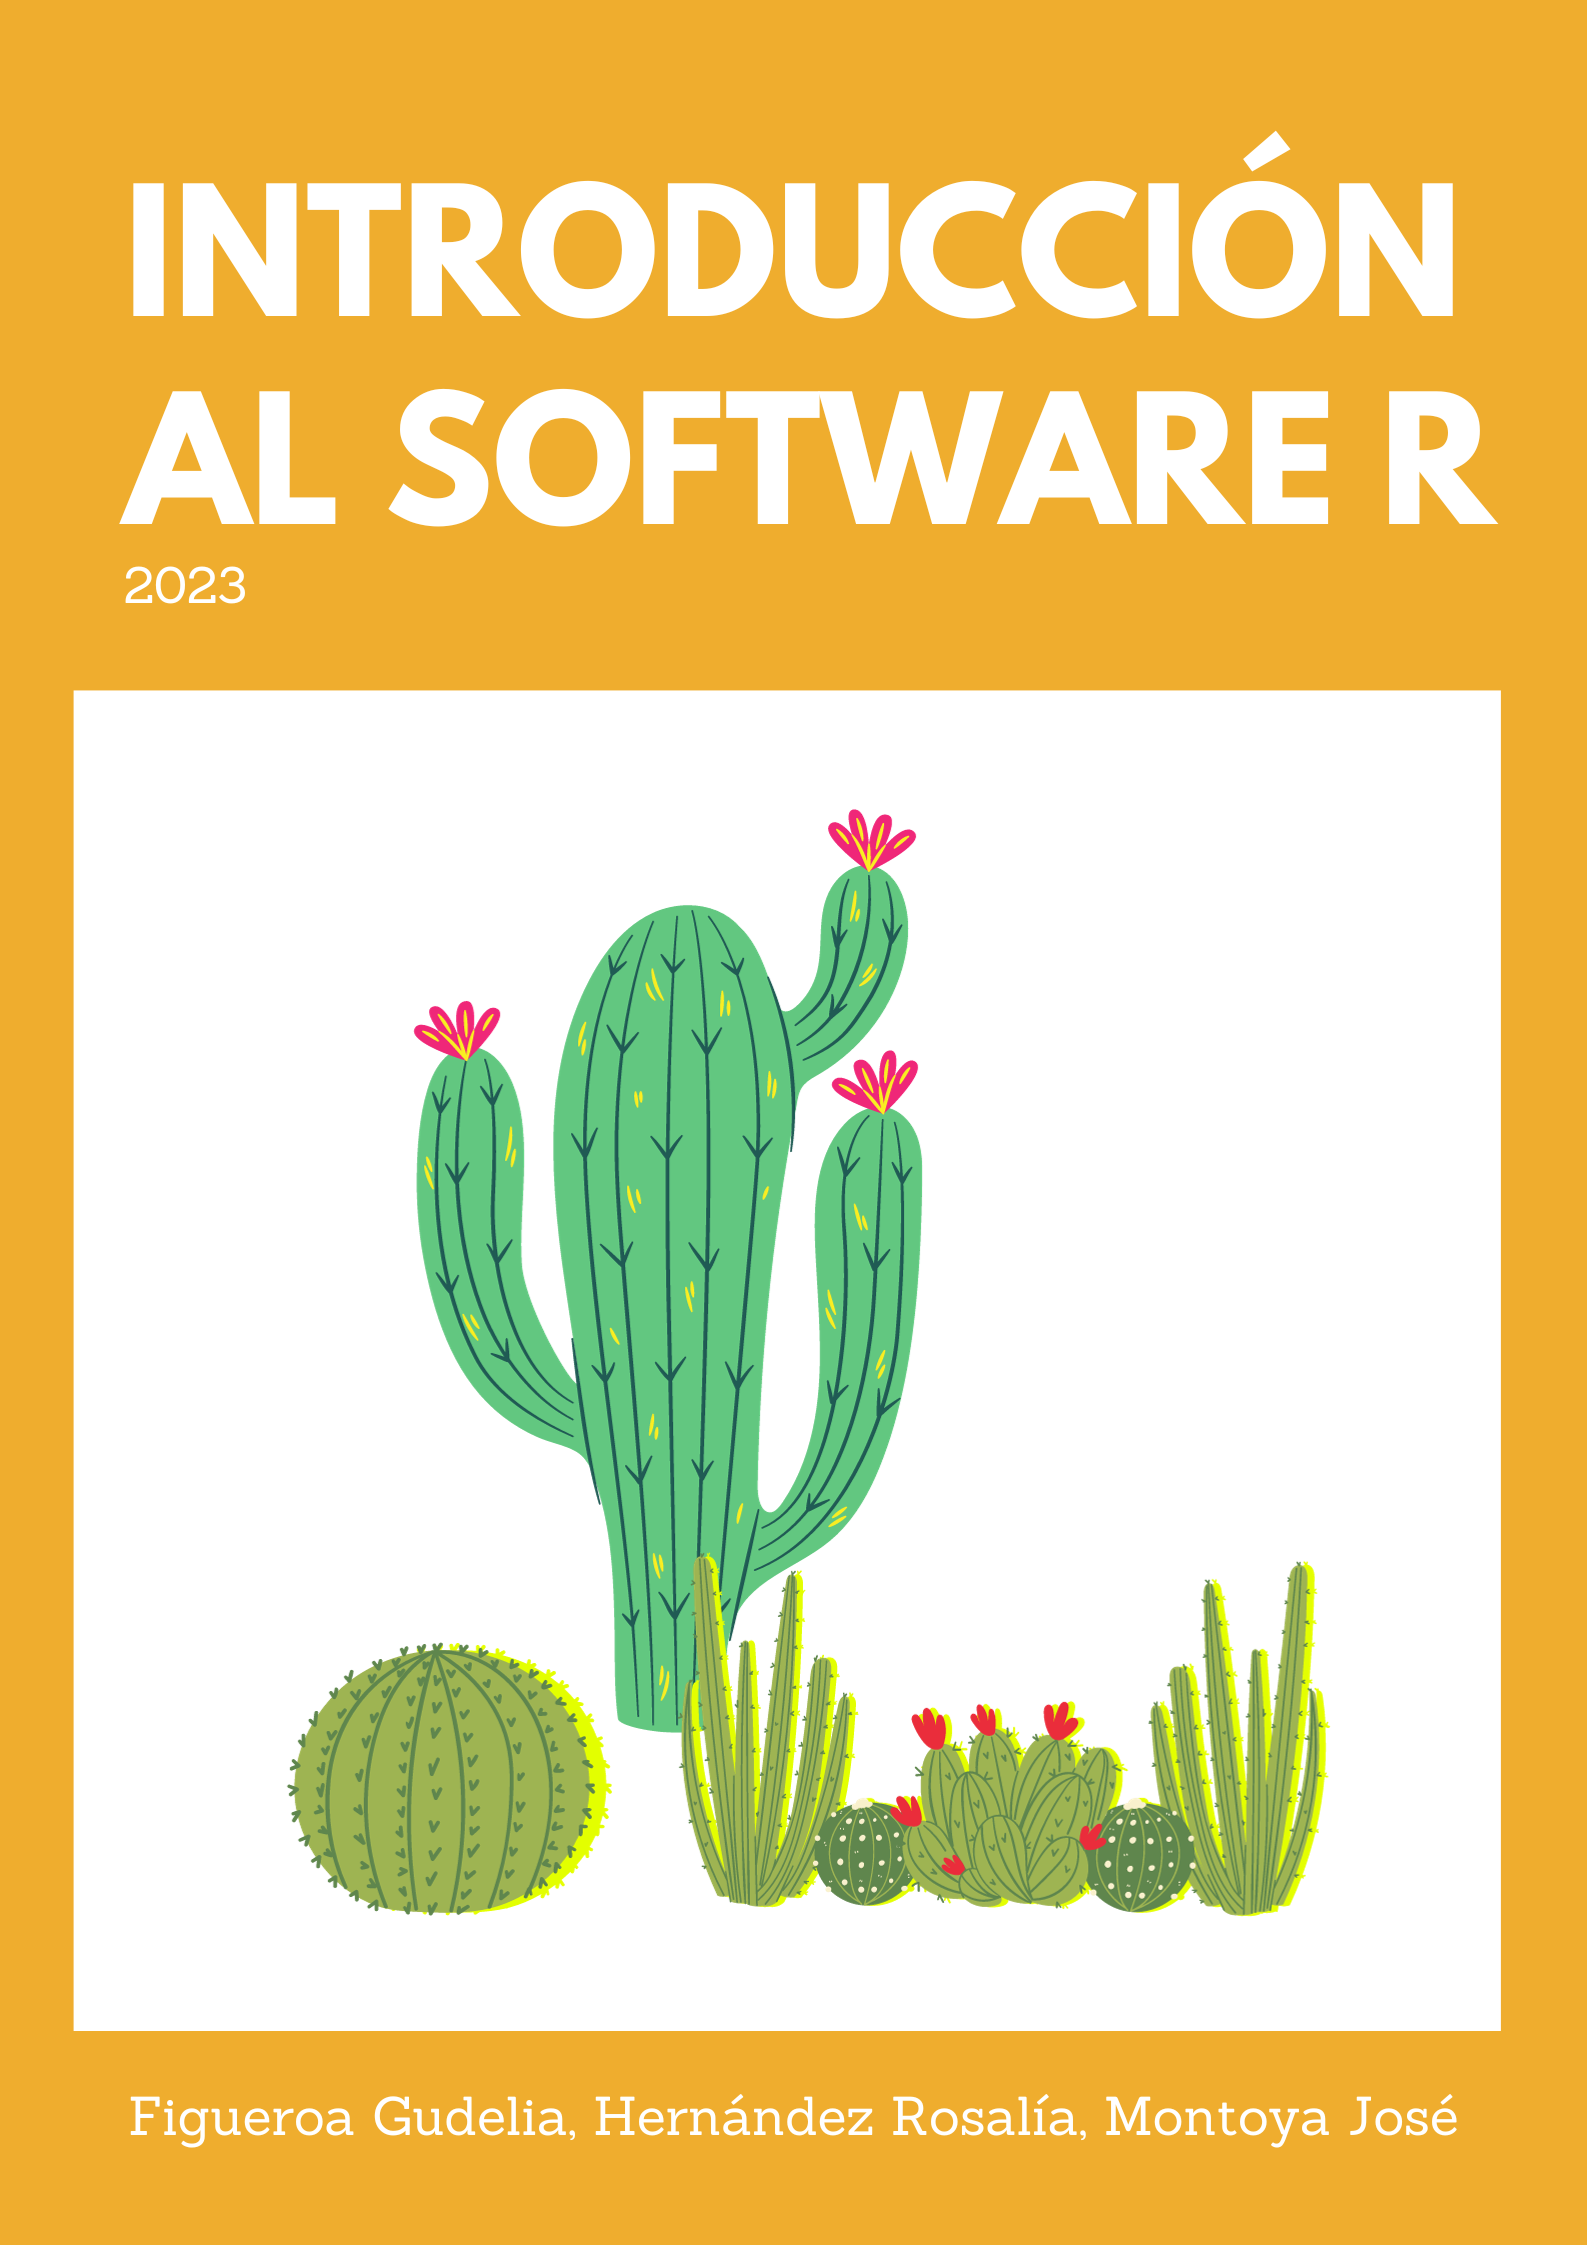
\includegraphics[width=4.10417in,height=\textheight]{portada.png}

Estas notas tienen el objetivo de proporcionar una introducción práctica al uso del software estadístico R, por medio de la interfaz gráfica RStudio.

Las notas fueron elaboradas como recurso de apoyo en el marco del \emph{Taller de Aplicación de técnicas estadísticas}, impartido a estudiantes del Posgrado en Biociencias de la Universidad de Sonora durante el semestre 2022-2, y fueron adaptadas para utilizarse en cursos de Estadística y Bioestadística durante los semestres 2023-1 y 2023-2 con estudiantes de nivel licenicatura.

Cabe mencionar que para los autores, resulta muy gratificante que las notas hayan sido puestas en práctica durante el mencionado taller por los distintos asistentes en sus proyectos de tesis, los cuales abarcan una amplia gama de temas en el área de Biociencias en problemáticas de gran relevancia e impacto regional, como estudios relativos a la dinámica y productividad de la flora y fauna en los distintos ecosistemas que se pueden encontrar en el estado de Sonora, desde las zonas desérticas a las costeras.

Los autores pretenden seguir enriqueciendo el texto con el uso subsecuente de las notas, y se espera que este trabajo sea una herramienta útil para los estudiantes que buscan comprender y aplicar las técnicas estadísticas en sus cursos y proyectos, propiciando la conexión entre la teoría y la práctica en esta disciplina.

\hypertarget{el-software}{%
\chapter{El software}\label{el-software}}

Estas notas ofrecen una introducción práctica al uso del software estadístico R mediante la interfaz gráfica RStudio. Es por ésto que para un mejor entendimiento de los conceptos y comandos que aquí se exponen, se exhorta al usuario a poner en práctica las instrucciones aquí documentadas.

\hypertarget{r-y-rstudio}{%
\section{R y RStudio}\label{r-y-rstudio}}

El software \textbf{R} es tanto un entorno de programación, como un lenguaje de programación, diseñado para hacer análisis estadístico. Es de código abierto, gratuito y multiplataforma, características que lo han convertido en una herramienta ampliamente utilizada en el campo de la estadística y el análisis de datos.

Por otro lado, \textbf{RStudio} es un entorno de desarrollo integrado (IDE) para trabajar con el lenguaje de programación R. Es una plataforma amigable para el usuario, y entre otras propiedades, facilita la escritura de código, visualización, generación de informes reproducibles y la exportación de resultados en diversos formatos.

El entorno RStudio, puede utilizarse de manera gratuita ingresando a través de una cuenta en Posit \url{https://posit.co/} o mediante la instalación previa de R y RStudio en gran variedad de sistemas operativos.

Para instalar R, podemos ingresar a la página \url{https://www.r-project.org} y descargar e instalar la última versión del software.

A continuación, para instalar RStudio, ingresamos a la página \url{https://www.posit.co} y descargamos e instalamos la interfaz gráfica RStudio.


\includegraphics{RyRStudio.png}

\hypertarget{rscripts}{%
\section{RScripts}\label{rscripts}}

Un \textbf{Rscript} es un archivo de texto compuesto de una serie de comandos e instrucciones escritos en el lenguaje de programación R, que al ser ejecutados realizan tareas específicas como leer y manipular datos, realizar análisis estadísticos o generar gráficos.

Una vez instalado RStudio, podemos abrir un RScript nuevo para escribir y documentar la secuencia de comandos que nos permitirá realizar alguna tarea determinada. Una buena práctica es incluir comentarios en este documento que describan lo que hace cada comando, y que nos permita documentar el código y facilitar su comprensión.

Los Rscripts permiten la reproducibilidad de los análisis resultantes, pues al guardar y compartir un Rscript con otros usuarios, éstos pueden ejecutar los mismos comandos para obtener resultados idénticos.

\hypertarget{libreruxeda-del-usuario}{%
\section{Librería del usuario}\label{libreruxeda-del-usuario}}

Al instalar el software R, se instala automáticamente una colección de \textbf{paquetes del sistema base}, que se almacenan en una librería. Estos paquetes se componen de funciones básicas del sistema que nos permiten realizar tareas comunes para la manipulación y el análisis de datos.

Adicionalmente, podemos instalar paquetes que nos permiten extender la funcionalidad del sistema base de R. Por ejemplo, podemos ampliar la capacidad de R para la generación de gráficos más atractivos, o para el análisis de datos en áreas especializadas como el estudio de series temporales, o para realizar análisis espaciales con el manejo de datos geoespaciales.

En el repositorio centralizado CRAN (Comprehensive R Archive Network) se albergan miles de paquetes creados por la comunidad de usuarios de R, disponibles para su descarga.

Para utilizar un paquete en R, primero debemos instalarlo y luego cargarlo en la sesión. Una vez cargado, podremos acceder a las funciones y capacidades que proporciona. A lo largo de este texto se explica el uso de una gran variedad de paquetes especializados para ejecutar ciertas tareas.

\hypertarget{datasets-integrados}{%
\section{Datasets integrados}\label{datasets-integrados}}

Existen algunos conjuntos de datos que se incluyen como parte de la instalación del sistema base de R, que se denominan \textbf{datasets}, los cuales son proporcionados por los desarrolladores del software y están disponibles para que los usuarios los utilicen directamente en su sesión, sin necesidad de descargar o importar datos desde fuentes externas.

Los datasets integrados en el sistema base de R son útiles para realizar ejemplos y pruebas, así como para aprender y practicar análisis de datos en R.

En estas notas se muestra el uso de algunas técnicas estadísticas aplicadas en datasets cargados en el sistema base de R.

\hypertarget{tipos-de-datos-y-objetos-en-r}{%
\chapter{Tipos de datos y objetos en R}\label{tipos-de-datos-y-objetos-en-r}}

R es un lenguaje de programación orientado a objetos, lo que significa que se centra en la manipulación de objetos y datos. Estos objetos nos permiten almacenar y manipular información.

Por ejemplo, en una \textbf{variable} podemos almacenar datos, los cuales pueden ser de distintos tipos como cadenas de caracteres, números enteros, números decimales, números complejos y valores lógicos (verdadero o falso).

Por otro lado, las \textbf{funciones} en R, son objetos que nos permiten manipular información para realizar operaciones específicas. Las funciones pueden tomar \textbf{argumentos o parámetros} que determinan cómo se ejecutan esas operaciones. Las funciones en R pueden ser funciones propias del lenguaje, o funciones definidas por el mismo usuario.

Se describen a continuación algunos otros objetos comunmente utilizados en R.

\hypertarget{vectores}{%
\section{Vectores}\label{vectores}}

Los \textbf{vectores} son una de las estructuras de datos más fundamentales en R. Un vector es una secuencia ordenada de elementos del mismo tipo, y pueden ser de tipo numérico, de caracteres, lógicos u otros tipos.

Por ejemplo, (0,1, 2, 3, 25, 23) es un vector numérico, que puede ser creado utilizando la función \texttt{c()} del sistema base de R la cual concatena elementos, y puede ser almacenado en la variable \texttt{x} mediante el símbolo de asignación \texttt{\textless{}-}:

\begin{Shaded}
\begin{Highlighting}[]
\NormalTok{x }\OtherTok{\textless{}{-}} \FunctionTok{c}\NormalTok{(}\DecValTok{0}\NormalTok{, }\DecValTok{1}\NormalTok{, }\DecValTok{2}\NormalTok{, }\DecValTok{3}\NormalTok{, }\DecValTok{25}\NormalTok{, }\DecValTok{23}\NormalTok{)}
\NormalTok{x}
\end{Highlighting}
\end{Shaded}

\begin{verbatim}
## [1]  0  1  2  3 25 23
\end{verbatim}

Podemos utilizar otras funciones para examinar distintas características de los objetos que creamos o que importamos. Por ejemplo, para verificar el tipo de objeto que almacenamos en la variable \texttt{x} podemos usar la función \texttt{class()},

\begin{Shaded}
\begin{Highlighting}[]
\FunctionTok{class}\NormalTok{(x)}
\end{Highlighting}
\end{Shaded}

\begin{verbatim}
## [1] "numeric"
\end{verbatim}

que indica que \texttt{x} es un vector numérico. Si además queremos investigar el tipo de datos que componen al objeto \texttt{x}, utilizamos la función \texttt{typeof()},

\begin{Shaded}
\begin{Highlighting}[]
\FunctionTok{typeof}\NormalTok{(x)}
\end{Highlighting}
\end{Shaded}

\begin{verbatim}
## [1] "double"
\end{verbatim}

que nos indica que los elementos numéricos son de hecho valores reales.

Otras características que podemos examinar es la longitud del vector,

\begin{Shaded}
\begin{Highlighting}[]
\FunctionTok{length}\NormalTok{(x)}
\end{Highlighting}
\end{Shaded}

\begin{verbatim}
## [1] 6
\end{verbatim}

o incluso podemos efectuar operaciones con los elementos almacenados en él, como por ejemplo, podemos sumar sus entradas con el comando \texttt{sum()}

\begin{Shaded}
\begin{Highlighting}[]
\FunctionTok{sum}\NormalTok{(x)}
\end{Highlighting}
\end{Shaded}

\begin{verbatim}
## [1] 54
\end{verbatim}

Otros ejemplos de vectores son:

\begin{Shaded}
\begin{Highlighting}[]
\NormalTok{y }\OtherTok{\textless{}{-}} \FunctionTok{c}\NormalTok{(}\StringTok{"A"}\NormalTok{, }\StringTok{"B"}\NormalTok{, }\StringTok{"C"}\NormalTok{) }\CommentTok{\# vector de caracteres}

\NormalTok{z }\OtherTok{\textless{}{-}} \FunctionTok{c}\NormalTok{(T, T, F, F) }\CommentTok{\# vector de elementos lógicos}

\NormalTok{w }\OtherTok{\textless{}{-}} \FunctionTok{c}\NormalTok{(}\DecValTok{5}\SpecialCharTok{:}\DecValTok{9}\NormalTok{) }\CommentTok{\# vector numérico con elementos enteros sucesivos del 5 al 9}
\end{Highlighting}
\end{Shaded}

Podemos también crear nuevos vectores a partir de otros dados, por ejemplo utilizando la función \texttt{rep()}

\begin{Shaded}
\begin{Highlighting}[]
\FunctionTok{rep}\NormalTok{(y, }\AttributeTok{times =} \DecValTok{4}\NormalTok{)}
\end{Highlighting}
\end{Shaded}

\begin{verbatim}
##  [1] "A" "B" "C" "A" "B" "C" "A" "B" "C" "A" "B" "C"
\end{verbatim}

instrucción con la que se ha concatenado 4 veces el vector \texttt{y}.

\hypertarget{matrices}{%
\section{Matrices}\label{matrices}}

Las \textbf{matrices} son estructuras bidimensionales en la que los datos están organizados en renglones y columnas. Todas las entradas de una matriz deben constar de elementos del mismo tipo de datos.

Por ejemplo, podemos manipular vectores para crear una matriz. Con la función \texttt{cbind()}, se pueden unir dos vectores para formar las columnas de una matriz

\begin{Shaded}
\begin{Highlighting}[]
\NormalTok{vec1 }\OtherTok{\textless{}{-}} \FunctionTok{c}\NormalTok{(}\DecValTok{1}\NormalTok{, }\DecValTok{2}\NormalTok{, }\DecValTok{3}\NormalTok{, }\DecValTok{4}\NormalTok{, }\DecValTok{5}\NormalTok{)}
\NormalTok{vec2 }\OtherTok{\textless{}{-}} \FunctionTok{c}\NormalTok{(}\SpecialCharTok{{-}}\DecValTok{1}\NormalTok{, }\SpecialCharTok{{-}}\DecValTok{2}\NormalTok{, }\SpecialCharTok{{-}}\DecValTok{3}\NormalTok{, }\SpecialCharTok{{-}}\DecValTok{4}\NormalTok{, }\SpecialCharTok{{-}}\DecValTok{5}\NormalTok{)}
\FunctionTok{cbind}\NormalTok{(}\AttributeTok{Columna\_1 =}\NormalTok{ vec1, }\AttributeTok{Columna\_2=}\NormalTok{ vec2)}
\end{Highlighting}
\end{Shaded}

\begin{verbatim}
##      Columna_1 Columna_2
## [1,]         1        -1
## [2,]         2        -2
## [3,]         3        -3
## [4,]         4        -4
## [5,]         5        -5
\end{verbatim}

o combinar por filas los vectores utilizando la función \texttt{rbind()}.

\begin{Shaded}
\begin{Highlighting}[]
\FunctionTok{rbind}\NormalTok{(}\AttributeTok{Renglon\_1 =}\NormalTok{ vec1,}\AttributeTok{Renglon\_2 =}\NormalTok{ vec2)}
\end{Highlighting}
\end{Shaded}

\begin{verbatim}
##           [,1] [,2] [,3] [,4] [,5]
## Renglon_1    1    2    3    4    5
## Renglon_2   -1   -2   -3   -4   -5
\end{verbatim}

\hypertarget{dataframes}{%
\section{Dataframes}\label{dataframes}}

Un \textbf{data frame} es una estructura bidimensional que se utiliza generalmente para almacenar datos tabulares. Cada columna de un data frame puede ser de un tipo diferente.

Los data frames son similares a las tablas de una base de datos u hojas de cálculo, donde las columnas representan variables, y los renglones corresponden a observaciones.

Existen algunos comandos que son especialmente útiles para indagar el contenido de una base de datos, especialmente cuando éstas son de gran tamaño.
Por ejemplo, supongamos que tenemos los tratamientos 1, 2 y 3, y que para cada uno de los tratamientos se utilizaron distintas unidades experimentales sobre las cuales se tomó una medición:

\begin{Shaded}
\begin{Highlighting}[]
\CommentTok{\# Almacenamos los datos en dos columnas}
\NormalTok{datos }\OtherTok{\textless{}{-}} \FunctionTok{data.frame}\NormalTok{(}\AttributeTok{Tratamiento =} \FunctionTok{rep}\NormalTok{(}\FunctionTok{c}\NormalTok{(}\StringTok{"1"}\NormalTok{, }\StringTok{"2"}\NormalTok{, }\StringTok{"3"}\NormalTok{), }\DecValTok{6}\NormalTok{), }
                    \AttributeTok{Tiempo =} \FunctionTok{c}\NormalTok{(}\DecValTok{14}\NormalTok{, }\DecValTok{16}\NormalTok{, }\DecValTok{13}\NormalTok{, }
                               \DecValTok{24}\NormalTok{, }\DecValTok{25}\NormalTok{, }\DecValTok{21}\NormalTok{, }
                               \DecValTok{18}\NormalTok{, }\DecValTok{19}\NormalTok{, }\DecValTok{14}\NormalTok{, }
                               \DecValTok{12}\NormalTok{, }\DecValTok{16}\NormalTok{, }\DecValTok{17}\NormalTok{, }
                               \DecValTok{23}\NormalTok{, }\DecValTok{22}\NormalTok{, }\DecValTok{21}\NormalTok{, }
                               \DecValTok{25}\NormalTok{, }\DecValTok{23}\NormalTok{, }\DecValTok{22}\NormalTok{)}
\NormalTok{                    )}
\NormalTok{datos}
\end{Highlighting}
\end{Shaded}

\begin{verbatim}
##    Tratamiento Tiempo
## 1            1     14
## 2            2     16
## 3            3     13
## 4            1     24
## 5            2     25
## 6            3     21
## 7            1     18
## 8            2     19
## 9            3     14
## 10           1     12
## 11           2     16
## 12           3     17
## 13           1     23
## 14           2     22
## 15           3     21
## 16           1     25
## 17           2     23
## 18           3     22
\end{verbatim}

Podemos analizar la estructura de la tabla utilizando la función \texttt{str()},

\begin{Shaded}
\begin{Highlighting}[]
\FunctionTok{str}\NormalTok{(datos)}
\end{Highlighting}
\end{Shaded}

\begin{verbatim}
## 'data.frame':    18 obs. of  2 variables:
##  $ Tratamiento: chr  "1" "2" "3" "1" ...
##  $ Tiempo     : num  14 16 13 24 25 21 18 19 14 12 ...
\end{verbatim}

que nos indica las características generales del dataframe, esto es, su tamaño, los nombres de las columnas, y el tipo de datos almacenados en cada columna.

Puede también ser útil visualizar los primeros renglones de la tabla, lo que podemos solicitar utilizando la función \texttt{head()},

\begin{Shaded}
\begin{Highlighting}[]
\CommentTok{\# Imprimir los primeros tres renglones del dataframe}
\FunctionTok{head}\NormalTok{(datos,}\DecValTok{3}\NormalTok{)}
\end{Highlighting}
\end{Shaded}

\begin{verbatim}
##   Tratamiento Tiempo
## 1           1     14
## 2           2     16
## 3           3     13
\end{verbatim}

y de manera similar, para visualizar lo últimos tres renglones, podmeos utilizar la función \texttt{tail()}

\begin{Shaded}
\begin{Highlighting}[]
\CommentTok{\# Imprimir los últimos tres renglones}
\FunctionTok{tail}\NormalTok{(datos,}\DecValTok{3}\NormalTok{)}
\end{Highlighting}
\end{Shaded}

\begin{verbatim}
##    Tratamiento Tiempo
## 16           1     25
## 17           2     23
## 18           3     22
\end{verbatim}

Al conocer el tipo de contenido de las bases de datos, tendremos un mejor entendiemiento de cómo manipular la información para realizar análisis más específicos.

\hypertarget{lectura-de-archivos}{%
\chapter{Lectura de archivos}\label{lectura-de-archivos}}

En R podemos importar una gran variedad de tipos de archivos, utilizando funciones propias del sistema base o funciones de otros paquetes.

Para leer bases de datos desde un archivo en nuestra computadora, debemos cuidar que éste se encuentre almacenado en el directorio de trabajo.

A continuación se describé cómo importar datos desde formatos de archivos más comunmente utilizados.

\hypertarget{archivos-de-texto}{%
\section{Archivos de texto}\label{archivos-de-texto}}

Para leer archivos en formato \textbf{TXT (texto plano)} podemos usar la función \texttt{read.delim()}:

\begin{Shaded}
\begin{Highlighting}[]
\NormalTok{Datostxt }\OtherTok{\textless{}{-}} \FunctionTok{read.delim}\NormalTok{(}\StringTok{"analgesics.txt"}\NormalTok{)}
\FunctionTok{head}\NormalTok{(Datostxt)}
\end{Highlighting}
\end{Shaded}

\begin{verbatim}
##   Pain_level Drug
## 1          4    A
## 2          5    A
## 3          4    A
## 4          3    A
## 5          2    A
## 6          4    A
\end{verbatim}

\hypertarget{archivos-csv}{%
\section{Archivos csv}\label{archivos-csv}}

Para leer archivos en formato \textbf{CSV (valores separados por comas)} podemos utilizar la función \texttt{read.csv},

\begin{Shaded}
\begin{Highlighting}[]
\NormalTok{Datoscsv }\OtherTok{\textless{}{-}} \FunctionTok{read.csv}\NormalTok{(}\StringTok{"calificaciones.csv"}\NormalTok{, }\AttributeTok{header =}\NormalTok{ T)}
\FunctionTok{head}\NormalTok{(Datoscsv)}
\end{Highlighting}
\end{Shaded}

\begin{verbatim}
##   X  id female race ses schtyp prog read write math science socst
## 1 1  70      0    4   1      1    1   57    52   41      47    57
## 2 2 121      1    4   2      1    3   68    59   53      63    61
## 3 3  86      0    4   3      1    1   44    33   54      58    31
## 4 4 141      0    4   3      1    3   63    44   47      53    56
## 5 5 172      0    4   2      1    2   47    52   57      53    61
## 6 6 113      0    4   2      1    2   44    52   51      63    61
\end{verbatim}

\hypertarget{archivos-de-excel}{%
\section{Archivos de Excel}\label{archivos-de-excel}}

Para importar datos desde archivos de Excel, en formato \textbf{XLSX (valores separados por tabulaciones)} podemos utilizar la función \texttt{read\_xlsx} del paquete \texttt{readxl}, que debemos agregar a la librería de usuario.

Para ésto descargamos primero el paquete, utilizando la función \texttt{install.packages()}, y a continuación lo cargamos a la sesión, para poder utilizar las funciones que contiene, utilizando el comando \texttt{library()}:

\begin{Shaded}
\begin{Highlighting}[]
\CommentTok{\# Instalación del paquete readxl}
\CommentTok{\# install.packages("readxl")}

\CommentTok{\# Carga del paquete en la sesión de trabajo}
\FunctionTok{library}\NormalTok{(readxl)}
\end{Highlighting}
\end{Shaded}

y posteriormente, leemos los datos,

\begin{Shaded}
\begin{Highlighting}[]
\NormalTok{DatosXlsx }\OtherTok{\textless{}{-}} \FunctionTok{read\_xlsx}\NormalTok{(}\StringTok{"Resultados.xlsx"}\NormalTok{)}
\end{Highlighting}
\end{Shaded}

\begin{verbatim}
## New names:
## * `` -> `...1`
\end{verbatim}

\begin{Shaded}
\begin{Highlighting}[]
\FunctionTok{head}\NormalTok{(DatosXlsx)}
\end{Highlighting}
\end{Shaded}

\begin{verbatim}
## # A tibble: 6 x 12
##    ...1    id female  race   ses schtyp  prog  read write  math science socst
##   <dbl> <dbl>  <dbl> <dbl> <dbl>  <dbl> <dbl> <dbl> <dbl> <dbl>   <dbl> <dbl>
## 1     1    70      0     4     1      1     1    57    52    41      47    57
## 2     2   121      1     4     2      1     3    68    59    53      63    61
## 3     3    86      0     4     3      1     1    44    33    54      58    31
## 4     4   141      0     4     3      1     3    63    44    47      53    56
## 5     5   172      0     4     2      1     2    47    52    57      53    61
## 6     6   113      0     4     2      1     2    44    52    51      63    61
\end{verbatim}

Para cada tipo de archivo, es posible encontrar funciones o paquetes específicos que facilitan su importación y el procesamiento de datos.

\hypertarget{anuxe1lisis-exploratorio-de-datos}{%
\chapter{Análisis exploratorio de datos}\label{anuxe1lisis-exploratorio-de-datos}}

Para comprender el comportamiento de un conjunto de datos, antes de aplicar técnicas más especializadas de la estadística, se suele realizar en primer lugar un análisis exploratprio de datos, con el objetivo de visualizar y comprender la distribución de los datos.

\hypertarget{ejemplo-1}{%
\section{Ejemplo 1}\label{ejemplo-1}}

Supongamos que registramos la cantidad de respuestas correctas logradas en un exámen, aplicado a un grupo de 15 estudiantes:

\begin{Shaded}
\begin{Highlighting}[]
\NormalTok{respuestas }\OtherTok{\textless{}{-}} \FunctionTok{c}\NormalTok{(}\DecValTok{2}\NormalTok{, }\DecValTok{4}\NormalTok{, }\DecValTok{4}\NormalTok{, }\DecValTok{3}\NormalTok{, }\DecValTok{5}\NormalTok{, }\DecValTok{5}\NormalTok{, }\DecValTok{6}\NormalTok{, }\DecValTok{3}\NormalTok{, }\DecValTok{7}\NormalTok{, }\DecValTok{8}\NormalTok{, }\DecValTok{3}\NormalTok{, }\DecValTok{4}\NormalTok{, }\DecValTok{5}\NormalTok{, }\DecValTok{5}\NormalTok{, }\DecValTok{4}\NormalTok{)}
\end{Highlighting}
\end{Shaded}

podemos crear una \textbf{tabla de frecuencias absolutas} con la siguiente instrucción:

\begin{Shaded}
\begin{Highlighting}[]
\FunctionTok{table}\NormalTok{(respuestas)}
\end{Highlighting}
\end{Shaded}

\begin{verbatim}
## respuestas
## 2 3 4 5 6 7 8 
## 1 3 4 4 1 1 1
\end{verbatim}

y elaborar una gráfica sencilla, pero de gran utilidad como lo es un \textbf{diagrama de barras}

\begin{Shaded}
\begin{Highlighting}[]
\FunctionTok{barplot}\NormalTok{(}\FunctionTok{table}\NormalTok{(respuestas), }
        \AttributeTok{main =} \StringTok{"Número de respuestas correctas"}\NormalTok{, }
        \AttributeTok{col =} \StringTok{"blue"}\NormalTok{)}
\end{Highlighting}
\end{Shaded}

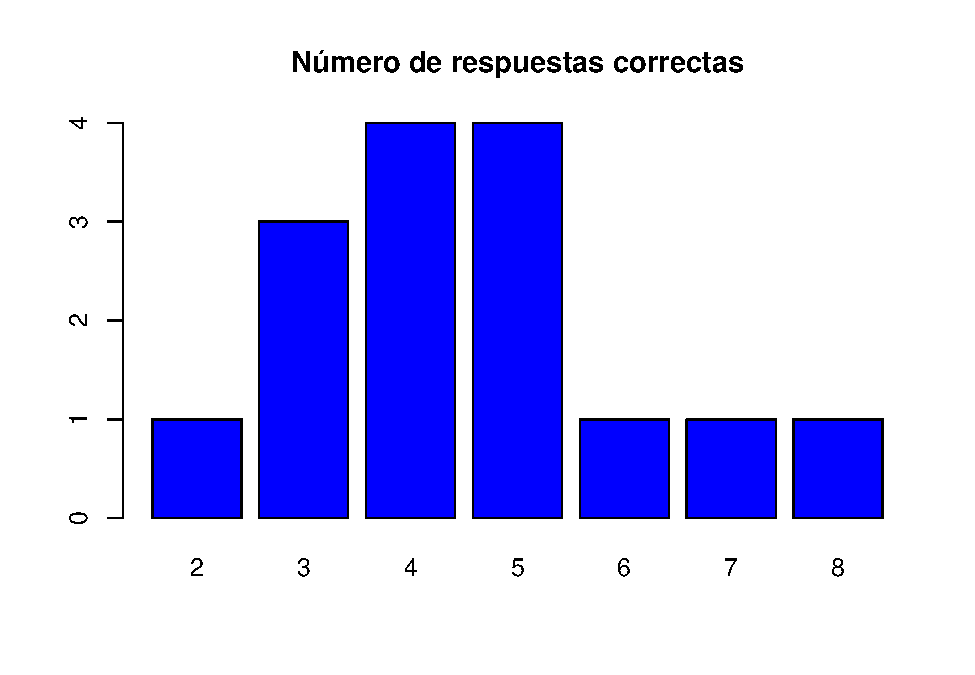
\includegraphics{_main_files/figure-latex/unnamed-chunk-20-1.pdf}

Además, podemos calcular fácilmente algunas medidas descriptivas. Por ejemplo, podemos examinar el valor mínimo y máximo ordenando las observaciones como sigue:

\begin{Shaded}
\begin{Highlighting}[]
\FunctionTok{sort}\NormalTok{(respuestas)}
\end{Highlighting}
\end{Shaded}

\begin{verbatim}
##  [1] 2 3 3 3 4 4 4 4 5 5 5 5 6 7 8
\end{verbatim}

calcular la \textbf{media},

\begin{Shaded}
\begin{Highlighting}[]
\FunctionTok{mean}\NormalTok{(respuestas)}
\end{Highlighting}
\end{Shaded}

\begin{verbatim}
## [1] 4.533333
\end{verbatim}

la \textbf{mediana},

\begin{Shaded}
\begin{Highlighting}[]
\FunctionTok{median}\NormalTok{(respuestas)}
\end{Highlighting}
\end{Shaded}

\begin{verbatim}
## [1] 4
\end{verbatim}

la \textbf{varianza},

\begin{Shaded}
\begin{Highlighting}[]
\FunctionTok{var}\NormalTok{(respuestas)}
\end{Highlighting}
\end{Shaded}

\begin{verbatim}
## [1] 2.552381
\end{verbatim}

la \textbf{desviación estándar},

\begin{Shaded}
\begin{Highlighting}[]
\FunctionTok{sd}\NormalTok{(respuestas)}
\end{Highlighting}
\end{Shaded}

\begin{verbatim}
## [1] 1.597617
\end{verbatim}

los \textbf{cuartiles},

\begin{Shaded}
\begin{Highlighting}[]
\FunctionTok{quantile}\NormalTok{(respuestas)}
\end{Highlighting}
\end{Shaded}

\begin{verbatim}
##   0%  25%  50%  75% 100% 
##  2.0  3.5  4.0  5.0  8.0
\end{verbatim}

especificar otros cuantiles deseados

\begin{Shaded}
\begin{Highlighting}[]
\FunctionTok{quantile}\NormalTok{(respuestas, }\FunctionTok{c}\NormalTok{(}\FloatTok{0.1}\NormalTok{,}\FloatTok{0.5}\NormalTok{,}\FloatTok{0.9}\NormalTok{))}
\end{Highlighting}
\end{Shaded}

\begin{verbatim}
## 10% 50% 90% 
## 3.0 4.0 6.6
\end{verbatim}

o podemos solicitar un resumen de las estadísticas descriptivas anteriores con la función \texttt{summary()},

\begin{Shaded}
\begin{Highlighting}[]
\FunctionTok{summary}\NormalTok{(respuestas)}
\end{Highlighting}
\end{Shaded}

\begin{verbatim}
##    Min. 1st Qu.  Median    Mean 3rd Qu.    Max. 
##   2.000   3.500   4.000   4.533   5.000   8.000
\end{verbatim}

\hypertarget{ejemplo-2}{%
\section{Ejemplo 2}\label{ejemplo-2}}

Consideremos ahora otro conjunto de datos,

\begin{Shaded}
\begin{Highlighting}[]
\NormalTok{datos2 }\OtherTok{\textless{}{-}} \FunctionTok{c}\NormalTok{(}\FloatTok{2.4}\NormalTok{, }\FloatTok{2.6}\NormalTok{, }\FloatTok{1.3}\NormalTok{, }\FloatTok{2.7}\NormalTok{, }\FloatTok{3.1}\NormalTok{, }\FloatTok{3.4}\NormalTok{, }\FloatTok{3.6}\NormalTok{, }\FloatTok{2.5}\NormalTok{, }\FloatTok{3.7}\NormalTok{, }
            \FloatTok{3.9}\NormalTok{, }\FloatTok{4.2}\NormalTok{, }\FloatTok{4.1}\NormalTok{, }\FloatTok{4.5}\NormalTok{, }\FloatTok{5.2}\NormalTok{, }\FloatTok{3.3}\NormalTok{, }\FloatTok{1.6}\NormalTok{, }\FloatTok{3.7}\NormalTok{,}\FloatTok{7.6}\NormalTok{)}
\end{Highlighting}
\end{Shaded}

Otra herramienta visual de la estadística descriptiva que podemos realizar en un conjunto de datos para analizar su distribución, es la construcción de un \textbf{diagrma de tallo y hojas}. Para elaborarlo, primero ordenamos los datos,

\begin{Shaded}
\begin{Highlighting}[]
\FunctionTok{sort}\NormalTok{(datos2)}
\end{Highlighting}
\end{Shaded}

\begin{verbatim}
##  [1] 1.3 1.6 2.4 2.5 2.6 2.7 3.1 3.3 3.4 3.6 3.7 3.7 3.9 4.1 4.2 4.5 5.2 7.6
\end{verbatim}

y graficamos el diagrama con los datos ordenados

\begin{Shaded}
\begin{Highlighting}[]
\FunctionTok{stem}\NormalTok{(datos2, }\AttributeTok{scale=}\DecValTok{2}\NormalTok{)}
\end{Highlighting}
\end{Shaded}

\begin{verbatim}
## 
##   The decimal point is at the |
## 
##   1 | 36
##   2 | 4567
##   3 | 1346779
##   4 | 125
##   5 | 2
##   6 | 
##   7 | 6
\end{verbatim}

o podemos elaborar también \textbf{un diagrama de caja},

\begin{Shaded}
\begin{Highlighting}[]
\FunctionTok{boxplot}\NormalTok{(datos2, }\AttributeTok{horizontal =}\NormalTok{ T, }\AttributeTok{border =} \StringTok{"blue"}\NormalTok{, }
        \AttributeTok{xlab =} \StringTok{"Tiempos"}\NormalTok{, }\AttributeTok{main =} \StringTok{"Diagrama de caja"}\NormalTok{)}
\end{Highlighting}
\end{Shaded}

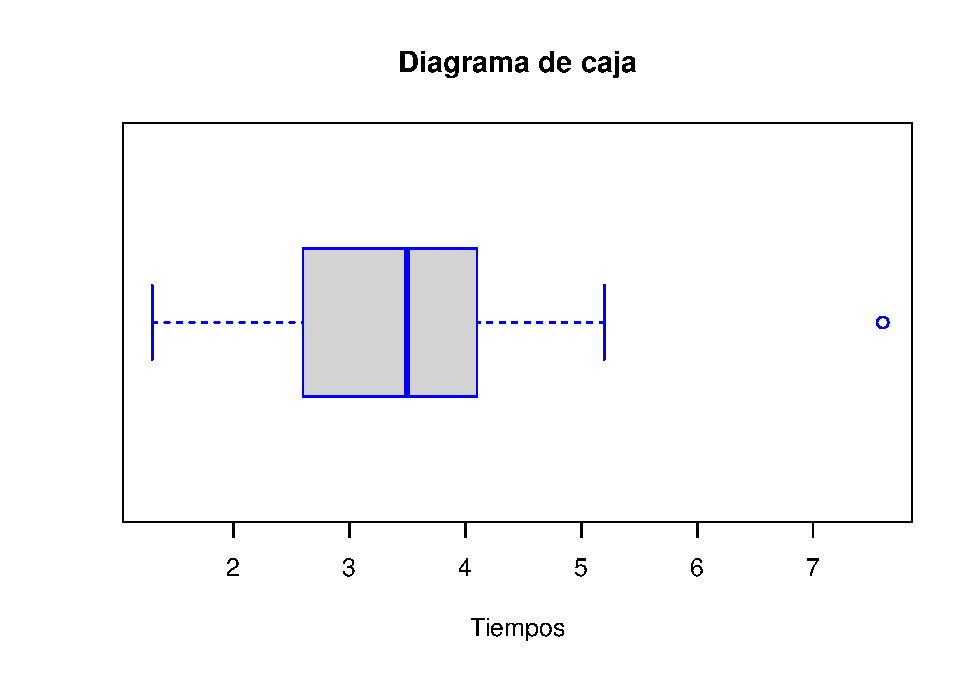
\includegraphics{_main_files/figure-latex/unnamed-chunk-32-1.pdf}

\hypertarget{ejemplo-3}{%
\section{Ejemplo 3}\label{ejemplo-3}}

Simulemos ahora una muestra aleatoria de 100 observaciones provenientes de una distribución normal, con media \(\mu = 20\) y desviación estándar \(\sigma = 3\),

\begin{Shaded}
\begin{Highlighting}[]
\NormalTok{datos3 }\OtherTok{\textless{}{-}} \FunctionTok{rnorm}\NormalTok{(}\DecValTok{100}\NormalTok{, }\DecValTok{20}\NormalTok{, }\DecValTok{3}\NormalTok{)}
\end{Highlighting}
\end{Shaded}

Podemos analizar su distribución por medio de un histograma,

\begin{Shaded}
\begin{Highlighting}[]
\FunctionTok{hist}\NormalTok{(datos3)}
\end{Highlighting}
\end{Shaded}

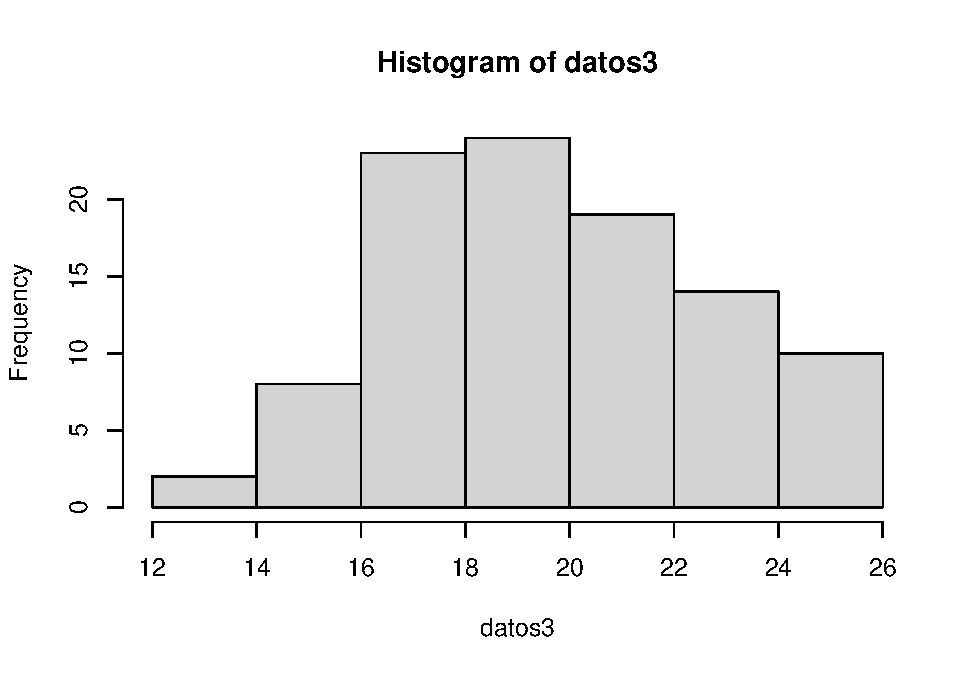
\includegraphics{_main_files/figure-latex/unnamed-chunk-34-1.pdf}

y personalizar la gráfica añadiendo una curva normal,

\begin{Shaded}
\begin{Highlighting}[]
\FunctionTok{hist}\NormalTok{(datos3, }\AttributeTok{freq =} \ConstantTok{FALSE}\NormalTok{)}
\NormalTok{ejenorm }\OtherTok{\textless{}{-}} \FunctionTok{seq}\NormalTok{(}\DecValTok{10}\NormalTok{, }\DecValTok{30}\NormalTok{, }\FloatTok{0.01}\NormalTok{)}
\FunctionTok{lines}\NormalTok{(ejenorm, }\FunctionTok{dnorm}\NormalTok{(ejenorm, }\DecValTok{20}\NormalTok{,}\DecValTok{3}\NormalTok{))}
\end{Highlighting}
\end{Shaded}

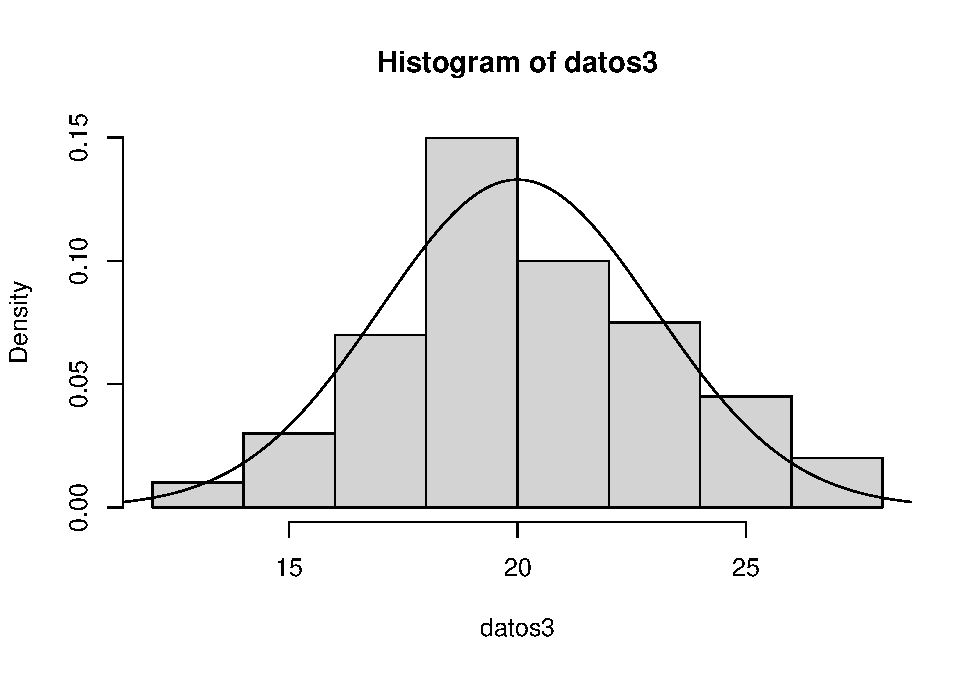
\includegraphics{_main_files/figure-latex/unnamed-chunk-35-1.pdf}

\hypertarget{ejemplo-4}{%
\section{Ejemplo 4}\label{ejemplo-4}}

Comparemos ahora varios conjuntos de datos. Para esto, generemos dos muestras de una distribución normal, y una tercer muestra de una distribución chi cuadarada,

\begin{Shaded}
\begin{Highlighting}[]
\NormalTok{x1 }\OtherTok{\textless{}{-}} \FunctionTok{rnorm}\NormalTok{(}\DecValTok{30}\NormalTok{, }\DecValTok{10}\NormalTok{, }\FloatTok{1.5}\NormalTok{)}
\NormalTok{x2 }\OtherTok{\textless{}{-}} \FunctionTok{rnorm}\NormalTok{(}\DecValTok{30}\NormalTok{, }\DecValTok{15}\NormalTok{, }\DecValTok{1}\NormalTok{)}
\NormalTok{x3 }\OtherTok{\textless{}{-}} \FunctionTok{rchisq}\NormalTok{(}\DecValTok{30}\NormalTok{, }\DecValTok{4}\NormalTok{)}
\end{Highlighting}
\end{Shaded}

Comparemos los datos de las primeras dos muestras mediante diagramas de cajas

\begin{Shaded}
\begin{Highlighting}[]
\FunctionTok{boxplot}\NormalTok{(x1,x2, }\AttributeTok{horizontal =} \ConstantTok{TRUE}\NormalTok{)}
\end{Highlighting}
\end{Shaded}

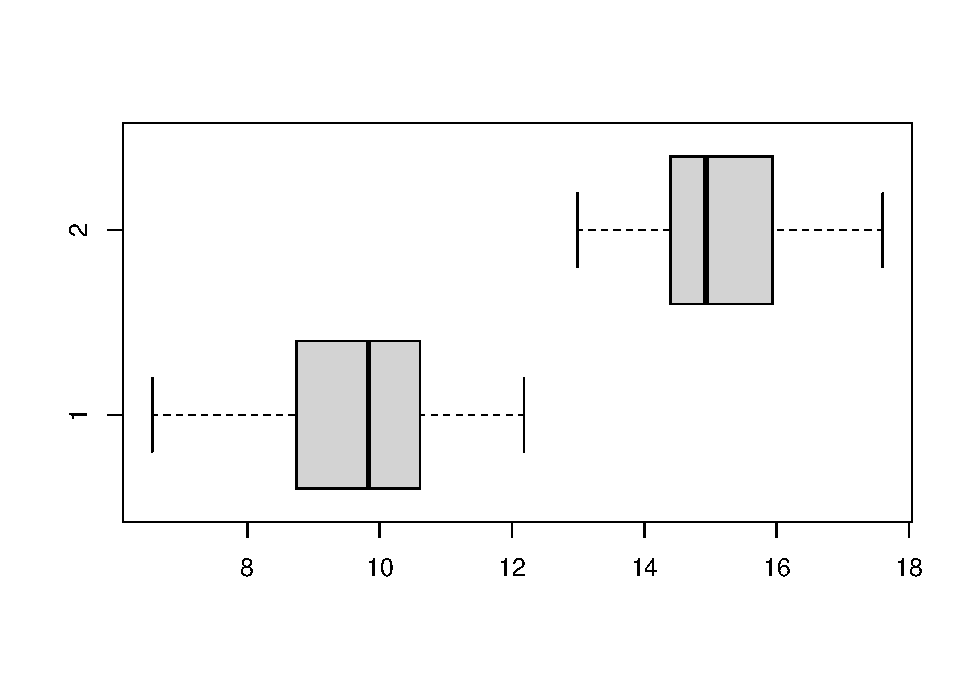
\includegraphics{_main_files/figure-latex/unnamed-chunk-37-1.pdf}

Podemos efectuar un \textbf{gráfico cuantil-cuantil (o gráfico Q-Q)}, para comparar si las dos muestras \texttt{x1} y \texttt{x2} provienen de la misma distribución

\begin{Shaded}
\begin{Highlighting}[]
\FunctionTok{qqplot}\NormalTok{(x1, x2, }\AttributeTok{xlim =} \FunctionTok{c}\NormalTok{(}\DecValTok{4}\NormalTok{,}\DecValTok{18}\NormalTok{), }\AttributeTok{ylim=}\FunctionTok{c}\NormalTok{(}\DecValTok{4}\NormalTok{,}\DecValTok{18}\NormalTok{))}
\end{Highlighting}
\end{Shaded}

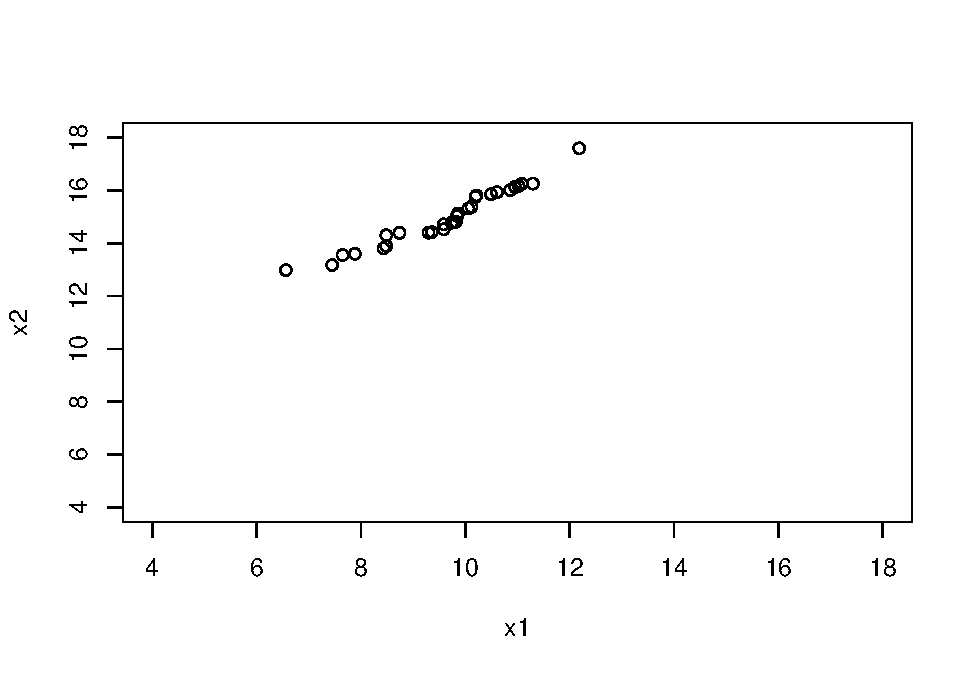
\includegraphics{_main_files/figure-latex/unnamed-chunk-38-1.pdf}

O podemos reemplazar una de las muestras en la comparación anterior, por los cuantiles de una distribución normal, para determinar si cada una de la muestras sigue una distribución normal. Por ejemplo, para la muestra \texttt{x1} obtenemos el siguiente gráfico,

\begin{Shaded}
\begin{Highlighting}[]
\FunctionTok{qqnorm}\NormalTok{(x1, }\AttributeTok{main=}\StringTok{"qqplot de x1"}\NormalTok{)}
\FunctionTok{qqline}\NormalTok{(x1,}\AttributeTok{col=}\DecValTok{2}\NormalTok{)}
\end{Highlighting}
\end{Shaded}

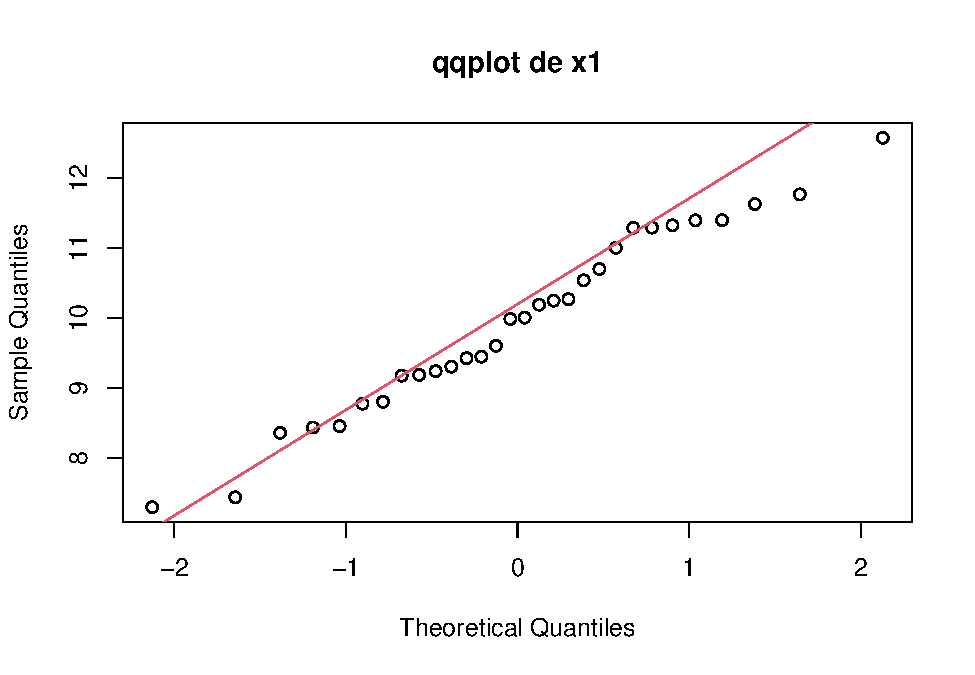
\includegraphics{_main_files/figure-latex/unnamed-chunk-39-1.pdf}

y para la muestra \texttt{x3} el siguiente,

\begin{Shaded}
\begin{Highlighting}[]
\FunctionTok{qqnorm}\NormalTok{(x3,}\AttributeTok{main=}\StringTok{"qqplot de x3"}\NormalTok{)}
\FunctionTok{qqline}\NormalTok{(x3,}\AttributeTok{col=}\DecValTok{2}\NormalTok{)}
\end{Highlighting}
\end{Shaded}

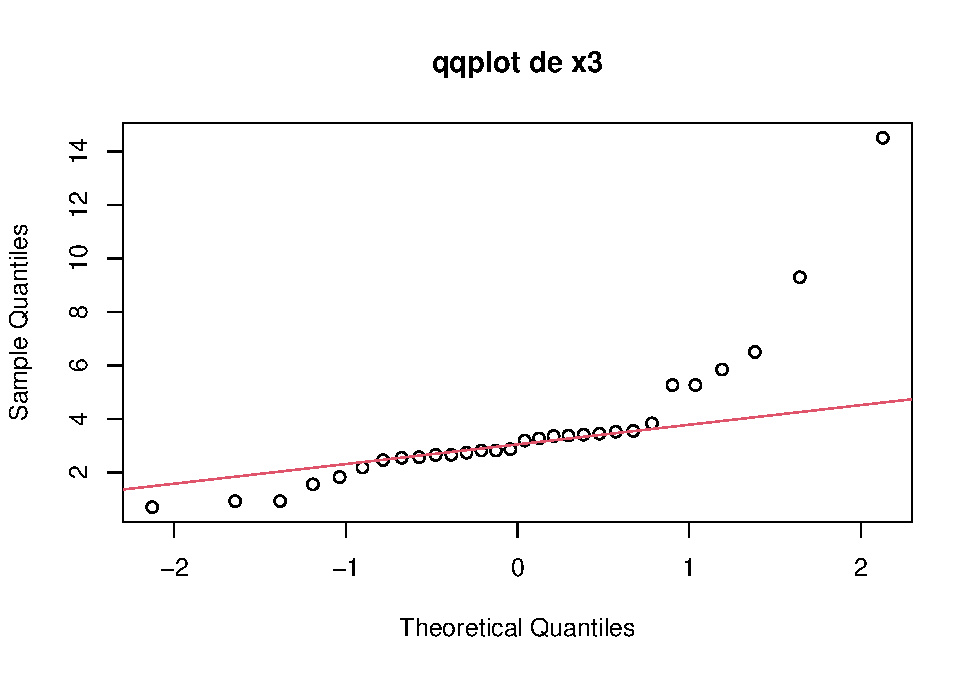
\includegraphics{_main_files/figure-latex/unnamed-chunk-40-1.pdf}

\hypertarget{anuxe1lisis-descriptivo-para-variables-correlacionadas}{%
\chapter{Análisis descriptivo para variables correlacionadas}\label{anuxe1lisis-descriptivo-para-variables-correlacionadas}}

Para comprender la relación entre dos variables y tomar decisiones sobre posibles análisis posteriores, un estudio común en estadística suele consistir en investigar si dos variables se encuentran correlacionadas. Usualmente se calcula un valor numérico de dicha correlación y se complementa el estudio con un análisis gráfico.

\hypertarget{ejemplo-1-1}{%
\section{Ejemplo 1}\label{ejemplo-1-1}}

Consideremos un experimento donde se registraron datos de la edad gestacional y peso al nacer de un grupo de 17 bebés.

\begin{Shaded}
\begin{Highlighting}[]
\NormalTok{edad\_ges }\OtherTok{\textless{}{-}} \FunctionTok{c}\NormalTok{(}\FloatTok{34.7}\NormalTok{, }\DecValTok{36}\NormalTok{,}\FloatTok{29.3}\NormalTok{, }\FloatTok{40.1}\NormalTok{, }\FloatTok{35.7}\NormalTok{, }\FloatTok{42.4}\NormalTok{, }\FloatTok{40.3}\NormalTok{, }\FloatTok{37.3}\NormalTok{, }\FloatTok{40.9}\NormalTok{, }
              \FloatTok{38.3}\NormalTok{, }\FloatTok{38.5}\NormalTok{, }\FloatTok{41.4}\NormalTok{, }\FloatTok{39.7}\NormalTok{, }\FloatTok{39.7}\NormalTok{, }\FloatTok{41.1}\NormalTok{, }\DecValTok{38}\NormalTok{, }\FloatTok{38.7}\NormalTok{)}

\NormalTok{peso\_nacer }\OtherTok{\textless{}{-}} \FunctionTok{c}\NormalTok{(}\DecValTok{1895}\NormalTok{, }\DecValTok{2030}\NormalTok{, }\DecValTok{1440}\NormalTok{, }\DecValTok{2835}\NormalTok{, }\DecValTok{3090}\NormalTok{, }\DecValTok{3827}\NormalTok{, }\DecValTok{3260}\NormalTok{, }\DecValTok{2690}\NormalTok{, }
                \DecValTok{3885}\NormalTok{, }\DecValTok{2920}\NormalTok{, }\DecValTok{3430}\NormalTok{, }\DecValTok{3657}\NormalTok{, }\DecValTok{3685}\NormalTok{, }\DecValTok{3345}\NormalTok{, }\DecValTok{3260}\NormalTok{, }\DecValTok{2680}\NormalTok{, }\DecValTok{2005}\NormalTok{)}
\end{Highlighting}
\end{Shaded}

Para comprender la relación entre estas dos variables, se puede calcular su \textbf{correlación},

\begin{Shaded}
\begin{Highlighting}[]
\FunctionTok{cor}\NormalTok{(edad\_ges,peso\_nacer)}
\end{Highlighting}
\end{Shaded}

\begin{verbatim}
## [1] 0.8197466
\end{verbatim}

y reforzar el resultado numérico obtenido, mediante un \textbf{diagrama de dispersión}

\begin{Shaded}
\begin{Highlighting}[]
\FunctionTok{plot}\NormalTok{(edad\_ges,peso\_nacer)}
\end{Highlighting}
\end{Shaded}

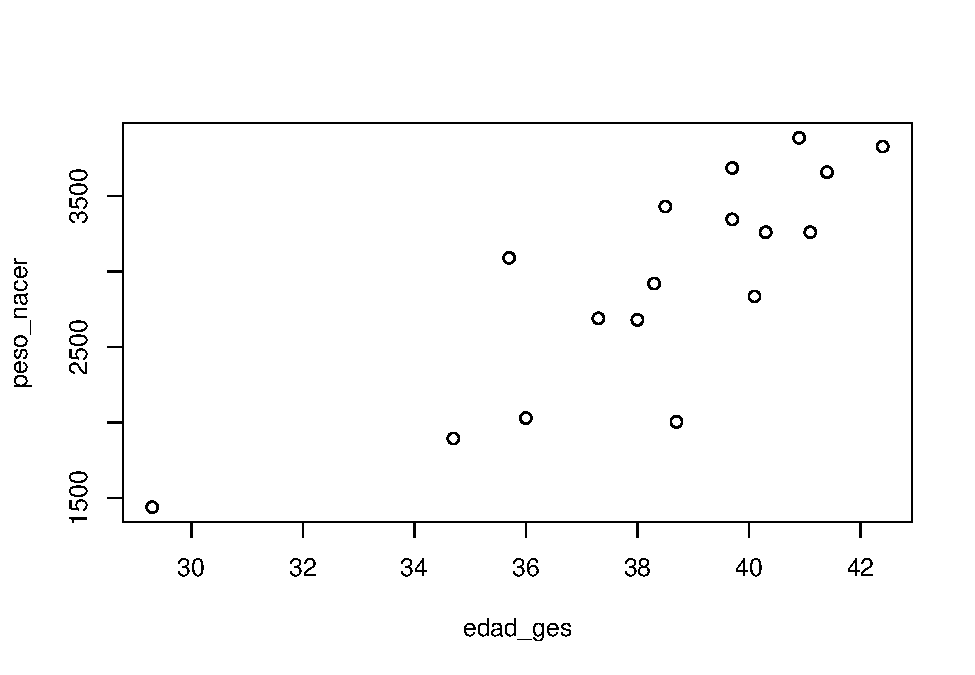
\includegraphics{_main_files/figure-latex/unnamed-chunk-43-1.pdf}

Podemos ajustar un modelo de \textbf{regresión lineal}, para establecer la relación lineal de una variable respecto a la otra,

\begin{Shaded}
\begin{Highlighting}[]
\NormalTok{reg1 }\OtherTok{\textless{}{-}} \FunctionTok{lm}\NormalTok{(peso\_nacer }\SpecialCharTok{\textasciitilde{}}\NormalTok{ edad\_ges)}
\end{Highlighting}
\end{Shaded}

y solicitar los detalles del modelo con la siguiente instrucción,

\begin{Shaded}
\begin{Highlighting}[]
\FunctionTok{summary}\NormalTok{(reg1) }
\end{Highlighting}
\end{Shaded}

\begin{verbatim}
## 
## Call:
## lm(formula = peso_nacer ~ edad_ges)
## 
## Residuals:
##     Min      1Q  Median      3Q     Max 
## -997.12 -198.17   -6.12  224.06  657.93 
## 
## Coefficients:
##             Estimate Std. Error t value Pr(>|t|)    
## (Intercept) -4351.62    1319.06  -3.299  0.00487 ** 
## edad_ges      190.02      34.28   5.543 5.63e-05 ***
## ---
## Signif. codes:  0 '***' 0.001 '**' 0.01 '*' 0.05 '.' 0.1 ' ' 1
## 
## Residual standard error: 432.8 on 15 degrees of freedom
## Multiple R-squared:  0.672,  Adjusted R-squared:  0.6501 
## F-statistic: 30.73 on 1 and 15 DF,  p-value: 5.629e-05
\end{verbatim}

podemos además ajustar la línea de regresión en el diagrama de dispersión,

\begin{Shaded}
\begin{Highlighting}[]
\FunctionTok{plot}\NormalTok{(edad\_ges,peso\_nacer)}
\FunctionTok{abline}\NormalTok{(reg1)}
\end{Highlighting}
\end{Shaded}

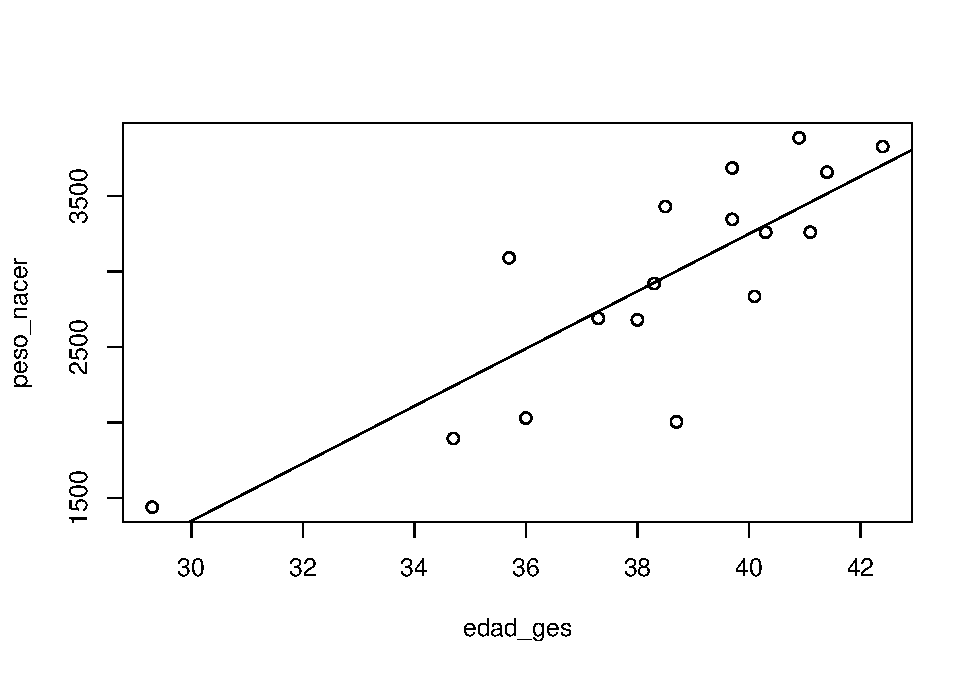
\includegraphics{_main_files/figure-latex/unnamed-chunk-46-1.pdf}

Para extraer información específica asociada al modelo, como por ejemplo sus coeficientes, podemos usar la siguiente instrucción,

\begin{Shaded}
\begin{Highlighting}[]
\NormalTok{reg1}\SpecialCharTok{$}\NormalTok{coefficients}
\end{Highlighting}
\end{Shaded}

\begin{verbatim}
## (Intercept)    edad_ges 
##  -4351.6240    190.0193
\end{verbatim}

y analizar el comportamiento de los residuales gráficamente

\begin{Shaded}
\begin{Highlighting}[]
\FunctionTok{plot}\NormalTok{(reg1}\SpecialCharTok{$}\NormalTok{residuals)}
\FunctionTok{abline}\NormalTok{(}\AttributeTok{h=}\DecValTok{0}\NormalTok{)}
\end{Highlighting}
\end{Shaded}

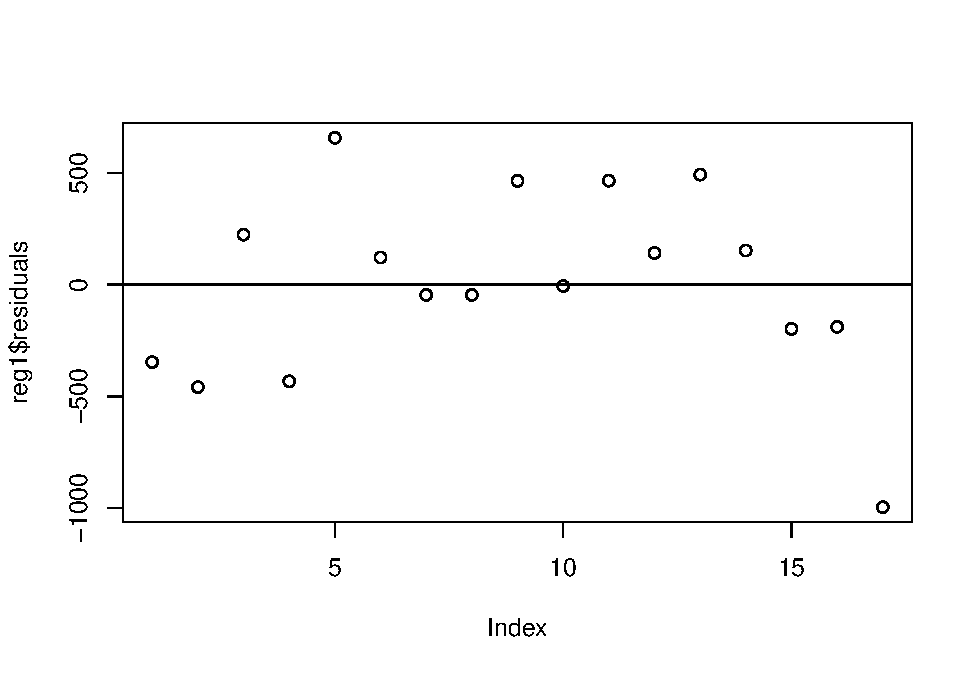
\includegraphics{_main_files/figure-latex/unnamed-chunk-48-1.pdf}

\hypertarget{ejemplo-2-1}{%
\section{Ejemplo 2}\label{ejemplo-2-1}}

A manera de ilustración del uso de datasets integrados en R, y para destacar la importancia de analizar un conjunto de datos desde diferentes perspectivas, a continuación se analiza el dataset \texttt{Anscombre}, el cual fué creado por el estadístico Francis Ascombre y publicado en 1973 en The American Statistician.

En primer lugar cargamos el conjunto de datos Anscombe,

\begin{Shaded}
\begin{Highlighting}[]
\FunctionTok{data}\NormalTok{(anscombe)}
\end{Highlighting}
\end{Shaded}

y podemos mostrar el contenido del dataset

\begin{Shaded}
\begin{Highlighting}[]
\NormalTok{anscombe}
\end{Highlighting}
\end{Shaded}

\begin{verbatim}
##    x1 x2 x3 x4    y1   y2    y3    y4
## 1  10 10 10  8  8.04 9.14  7.46  6.58
## 2   8  8  8  8  6.95 8.14  6.77  5.76
## 3  13 13 13  8  7.58 8.74 12.74  7.71
## 4   9  9  9  8  8.81 8.77  7.11  8.84
## 5  11 11 11  8  8.33 9.26  7.81  8.47
## 6  14 14 14  8  9.96 8.10  8.84  7.04
## 7   6  6  6  8  7.24 6.13  6.08  5.25
## 8   4  4  4 19  4.26 3.10  5.39 12.50
## 9  12 12 12  8 10.84 9.13  8.15  5.56
## 10  7  7  7  8  4.82 7.26  6.42  7.91
## 11  5  5  5  8  5.68 4.74  5.73  6.89
\end{verbatim}

Como podemos observar, este dataset consta de cuatro subconjuntos de datos, con 11 pares de observaciones cada uno del tipo \((x_i,y_i), i = 1, ..., 4\).

Para poder utilizar en el análisis siguiente los nombres de las variables tal y como aparecen en la tabla, utilizamos la instrucción \texttt{attach()},

\begin{Shaded}
\begin{Highlighting}[]
\FunctionTok{rm}\NormalTok{(}\AttributeTok{list =} \FunctionTok{ls}\NormalTok{())}
\FunctionTok{attach}\NormalTok{(anscombe)}
\end{Highlighting}
\end{Shaded}

Como podemos ver con los siguientes cálculos, estos cuatro subconjuntos tienen propiedades estadísticas muy similares, pues si ajustamos un modelo de regresión a cada subconjunto, obtenemos lo siguiente:

\begin{Shaded}
\begin{Highlighting}[]
\NormalTok{regresion1 }\OtherTok{\textless{}{-}} \FunctionTok{lm}\NormalTok{(y1 }\SpecialCharTok{\textasciitilde{}}\NormalTok{ x1)}
\NormalTok{regresion1}
\end{Highlighting}
\end{Shaded}

\begin{verbatim}
## 
## Call:
## lm(formula = y1 ~ x1)
## 
## Coefficients:
## (Intercept)           x1  
##      3.0001       0.5001
\end{verbatim}

\begin{Shaded}
\begin{Highlighting}[]
\NormalTok{regresion2 }\OtherTok{\textless{}{-}} \FunctionTok{lm}\NormalTok{(y2 }\SpecialCharTok{\textasciitilde{}}\NormalTok{ x2)}
\NormalTok{regresion2}
\end{Highlighting}
\end{Shaded}

\begin{verbatim}
## 
## Call:
## lm(formula = y2 ~ x2)
## 
## Coefficients:
## (Intercept)           x2  
##       3.001        0.500
\end{verbatim}

\begin{Shaded}
\begin{Highlighting}[]
\NormalTok{regresion3 }\OtherTok{\textless{}{-}} \FunctionTok{lm}\NormalTok{(y3}\SpecialCharTok{\textasciitilde{}}\NormalTok{ x3)}
\NormalTok{regresion3}
\end{Highlighting}
\end{Shaded}

\begin{verbatim}
## 
## Call:
## lm(formula = y3 ~ x3)
## 
## Coefficients:
## (Intercept)           x3  
##      3.0025       0.4997
\end{verbatim}

\begin{Shaded}
\begin{Highlighting}[]
\NormalTok{regresion4 }\OtherTok{\textless{}{-}} \FunctionTok{lm}\NormalTok{(y4}\SpecialCharTok{\textasciitilde{}}\NormalTok{x4)}
\NormalTok{regresion4}
\end{Highlighting}
\end{Shaded}

\begin{verbatim}
## 
## Call:
## lm(formula = y4 ~ x4)
## 
## Coefficients:
## (Intercept)           x4  
##      3.0017       0.4999
\end{verbatim}

sin embargo, al momento de representar gráficamente el comportamiento de los cuatro conjuntos de datos mediante diagramas de dispersión, podemos comprobar que difieren significativamente

\begin{Shaded}
\begin{Highlighting}[]
\FunctionTok{par}\NormalTok{(}\AttributeTok{mfrow =} \FunctionTok{c}\NormalTok{(}\DecValTok{2}\NormalTok{,}\DecValTok{2}\NormalTok{))}
\FunctionTok{plot}\NormalTok{(x1,y1)}
\FunctionTok{plot}\NormalTok{(x2,y2)}
\FunctionTok{plot}\NormalTok{(x3,y3)}
\FunctionTok{plot}\NormalTok{(x4,y4)}
\end{Highlighting}
\end{Shaded}

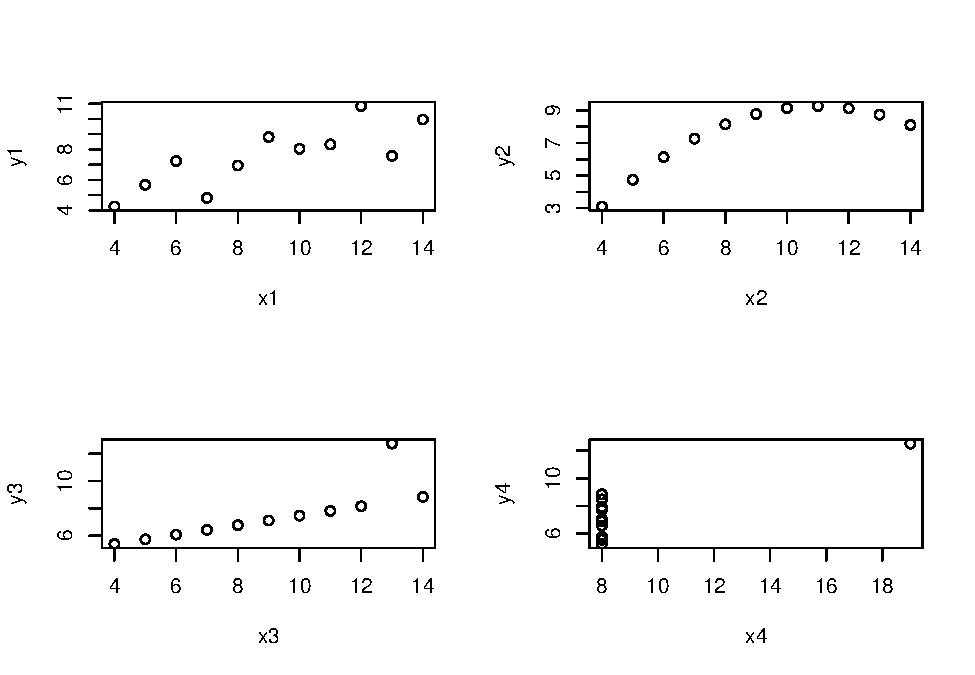
\includegraphics{_main_files/figure-latex/unnamed-chunk-56-1.pdf}

Este conjunto de datos, precargado en R, es un ejemplo claro de la importancia de la visualización de datos en el análisis estadístico.

\hypertarget{intervalos-de-confianza}{%
\chapter{Intervalos de confianza}\label{intervalos-de-confianza}}

Un intervalo de confianza es un rango de valores que se utiliza en estadística para estimar un parámetro desconocido de una población en base a una muestra de datos. Comunmente el parámetro desconocido es la media, una proporción o la varianza. Su objetivo es para proporcionar una medida de la incertidumbre asociada con la estimación del parámetro en cuestión.

La intención del siguiente ejercicio es comprender el significado de nivel de confianza \(1-\alpha\) de un intervalo de confianza.

Para ésto, se simulan a continuación 25 muestras de tamaño 20 cada una, de datos provenientes de una distribución normal con media \(\mu = 10\) y desviación estándar \(\sigma = 2\).

Para cada una de las muestras se calcula un \textbf{intervalo de confianza} del \(95\)\% para la media \(\mu\), utilizando un estadístico \(t\)-Student. Por medio de una gráfica se explora cuántos de estos intervalos capturaron el verdadero valor de \(\mu =10\):

\begin{Shaded}
\begin{Highlighting}[]
\NormalTok{mu }\OtherTok{\textless{}{-}} \DecValTok{10} \CommentTok{\# media}
\NormalTok{sigma }\OtherTok{\textless{}{-}} \DecValTok{2} \CommentTok{\# desviación estándar}
\NormalTok{n }\OtherTok{\textless{}{-}} \DecValTok{20} \CommentTok{\# tamaño de muestra}
\NormalTok{m }\OtherTok{\textless{}{-}} \DecValTok{25} \CommentTok{\# cantidad de muestras}

\CommentTok{\# inicializamos vectores vacíos}
\NormalTok{pvalor }\OtherTok{\textless{}{-}} \FunctionTok{rep}\NormalTok{(}\ConstantTok{NA}\NormalTok{,m) }
\NormalTok{resultado1 }\OtherTok{\textless{}{-}} \FunctionTok{rep}\NormalTok{(}\ConstantTok{NA}\NormalTok{,m)}
\NormalTok{resultado2 }\OtherTok{\textless{}{-}} \FunctionTok{rep}\NormalTok{(}\ConstantTok{NA}\NormalTok{,m)}
\NormalTok{medias }\OtherTok{\textless{}{-}} \FunctionTok{rep}\NormalTok{(}\ConstantTok{NA}\NormalTok{,m)}

\CommentTok{\# Repetir m veces el procedimiento}
\ControlFlowTok{for}\NormalTok{(i }\ControlFlowTok{in} \DecValTok{1}\SpecialCharTok{:}\NormalTok{m)}
\NormalTok{\{}
\NormalTok{  x }\OtherTok{\textless{}{-}} \FunctionTok{rnorm}\NormalTok{(n,mu,sigma)}
\NormalTok{  medias[i] }\OtherTok{\textless{}{-}} \FunctionTok{mean}\NormalTok{(x)}
\NormalTok{  pvalor[i] }\OtherTok{\textless{}{-}} \FunctionTok{t.test}\NormalTok{(x, }\AttributeTok{alternative =} \StringTok{"two.sided"}\NormalTok{, }
                      \AttributeTok{mu=}\DecValTok{10}\NormalTok{)}\SpecialCharTok{$}\NormalTok{p.value}
\NormalTok{  resultado1[i] }\OtherTok{\textless{}{-}} \FunctionTok{t.test}\NormalTok{(x, }\AttributeTok{alternative =} \StringTok{"two.sided"}\NormalTok{,}
                          \AttributeTok{mu=}\DecValTok{10}\NormalTok{)}\SpecialCharTok{$}\NormalTok{conf.int[}\DecValTok{1}\NormalTok{]}
\NormalTok{  resultado2[i] }\OtherTok{\textless{}{-}} \FunctionTok{t.test}\NormalTok{(x, }\AttributeTok{alternative =} \StringTok{"two.sided"}\NormalTok{,}
                          \AttributeTok{mu=}\DecValTok{10}\NormalTok{)}\SpecialCharTok{$}\NormalTok{conf.int[}\DecValTok{2}\NormalTok{]}
\NormalTok{\}}

\CommentTok{\# Cargamos el paquete plotrix}
\FunctionTok{library}\NormalTok{(plotrix)}

\CommentTok{\# Usamos la función plotCI() del paquete plotrix para graficar los IC}
\FunctionTok{plotCI}\NormalTok{(pvalor, medias, }\AttributeTok{ui =}\NormalTok{ resultado2, }\AttributeTok{li =}\NormalTok{ resultado1, }
       \AttributeTok{yab =}\StringTok{"Intervalos al 95\% de confianza"}\NormalTok{)}
\FunctionTok{abline}\NormalTok{(}\AttributeTok{h=}\NormalTok{mu,}\AttributeTok{col=}\StringTok{"blue"}\NormalTok{)}
\end{Highlighting}
\end{Shaded}

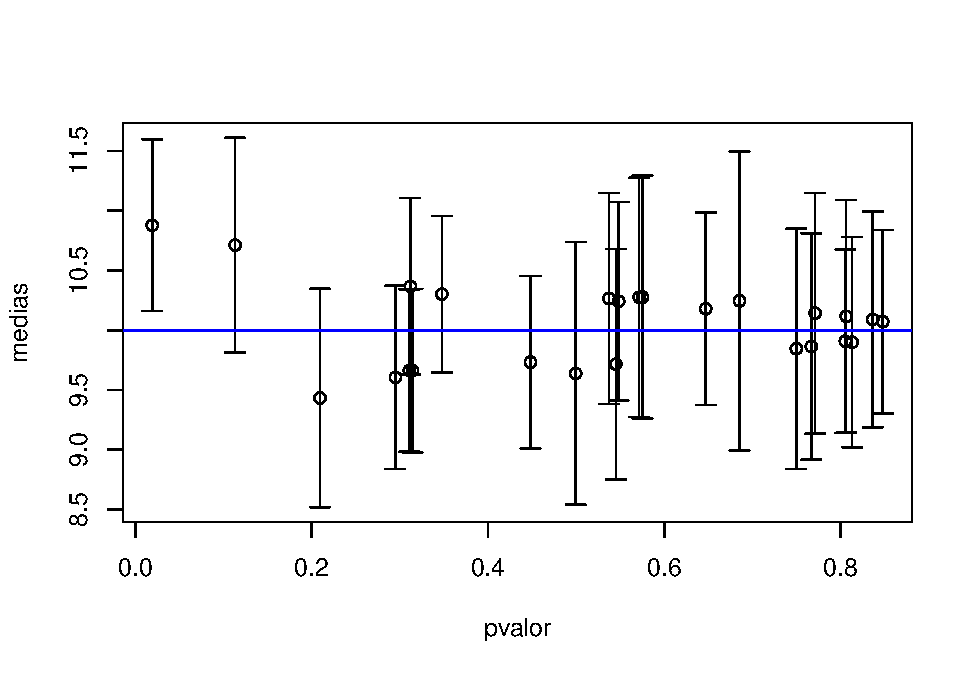
\includegraphics{_main_files/figure-latex/unnamed-chunk-57-1.pdf}

y podemos detallar la información sobre los 25 intervalos,

\begin{Shaded}
\begin{Highlighting}[]
\NormalTok{resultgral }\OtherTok{\textless{}{-}} \FunctionTok{cbind}\NormalTok{(pvalor, resultado1,resultado2)}
\NormalTok{resultgral}
\end{Highlighting}
\end{Shaded}

\begin{verbatim}
##          pvalor resultado1 resultado2
##  [1,] 0.3477809   9.646192   10.95651
##  [2,] 0.8063723   9.142150   11.08905
##  [3,] 0.6853893   8.995020   11.49669
##  [4,] 0.5450618   8.751950   10.68031
##  [5,] 0.4482927   9.011083   10.45483
##  [6,] 0.7710948   9.134454   11.14971
##  [7,] 0.8131286   9.020261   10.77839
##  [8,] 0.8478618   9.303247   10.83950
##  [9,] 0.4995012   8.541457   10.73654
## [10,] 0.5753673   9.260954   11.29221
## [11,] 0.0192584  10.159395   11.59655
## [12,] 0.5482903   9.412414   11.07234
## [13,] 0.3144359   8.978627   10.34621
## [14,] 0.8054629   9.140702   10.67609
## [15,] 0.8365133   9.187201   10.99333
## [16,] 0.1132281   9.814496   11.60982
## [17,] 0.7667446   8.916962   10.81076
## [18,] 0.7498114   8.840841   10.84876
## [19,] 0.2951013   8.839982   10.37195
## [20,] 0.2095819   8.519360   10.34675
## [21,] 0.3109084   8.983693   10.34112
## [22,] 0.6470200   9.373389   10.98484
## [23,] 0.5715428   9.274720   11.27571
## [24,] 0.5373050   9.381629   11.14884
## [25,] 0.3121481   9.627332   11.10645
\end{verbatim}

Si contamos la cantidad de veces que los intervalos capturaron el valor real \(\mu=10\),

\begin{Shaded}
\begin{Highlighting}[]
\NormalTok{cont}\OtherTok{=}\DecValTok{0}
\ControlFlowTok{for}\NormalTok{(i }\ControlFlowTok{in} \DecValTok{1}\SpecialCharTok{:}\NormalTok{m)}
\NormalTok{\{}
  \ControlFlowTok{if}\NormalTok{(mu}\SpecialCharTok{\textgreater{}}\NormalTok{ resultado1[i] }\SpecialCharTok{\&\&}\NormalTok{ mu }\SpecialCharTok{\textless{}}\NormalTok{ resultado2[i])}
\NormalTok{    cont}\OtherTok{=}\NormalTok{cont}\SpecialCharTok{+}\DecValTok{1}
\NormalTok{\}}
\NormalTok{cont}
\end{Highlighting}
\end{Shaded}

\begin{verbatim}
## [1] 24
\end{verbatim}

y calculamos la proporción de veces que ésto ocurre,

\begin{Shaded}
\begin{Highlighting}[]
\NormalTok{cont}\SpecialCharTok{/}\DecValTok{25}
\end{Highlighting}
\end{Shaded}

\begin{verbatim}
## [1] 0.96
\end{verbatim}

podemos ver es un valor muy cercano al 95\%.

\hypertarget{intervalo-de-confianza-y-prueba-de-hipuxf3tesis-para-comparar-dos-medias}{%
\chapter{Intervalo de confianza y prueba de hipótesis para comparar dos medias}\label{intervalo-de-confianza-y-prueba-de-hipuxf3tesis-para-comparar-dos-medias}}

La comparación de dos medias es un procedimiento común en estadística que se utiliza cuando se desea determinar si existen diferencias significativas entre las medias de dos grupos o poblaciones. El siguiente ejercicio muestra dos enfoques para la comparación de medias, mediante intervalos de confianza y mediante pruebas de hipótesis.

Para este tipo de procedimientos, debemos verificar primeramente que se cumplen los supuestos de normalidad en las muestras que se asumen independientes, y debemos verificar que no sea rechazado el supuesto de homogeneidad de varianzas.

Consideremos dos muestras independientes de datos:

\begin{Shaded}
\begin{Highlighting}[]
\FunctionTok{rm}\NormalTok{(}\AttributeTok{list=}\FunctionTok{ls}\NormalTok{())}
\NormalTok{metodoA }\OtherTok{\textless{}{-}} \FunctionTok{c}\NormalTok{(}\FloatTok{23.2}\NormalTok{,}\FloatTok{26.6}\NormalTok{,}\FloatTok{24.4}\NormalTok{, }\FloatTok{23.5}\NormalTok{, }\FloatTok{22.6}\NormalTok{, }\FloatTok{25.7}\NormalTok{, }\FloatTok{25.5}\NormalTok{, }\FloatTok{22.3}\NormalTok{, }
             \FloatTok{22.5}\NormalTok{, }\FloatTok{23.1}\NormalTok{, }\FloatTok{24.6}\NormalTok{, }\FloatTok{25.2}\NormalTok{, }\FloatTok{23.7}\NormalTok{)}

\NormalTok{metodoB }\OtherTok{\textless{}{-}} \FunctionTok{c}\NormalTok{(}\FloatTok{25.7}\NormalTok{, }\FloatTok{27.7}\NormalTok{, }\FloatTok{26.2}\NormalTok{, }\FloatTok{27.9}\NormalTok{, }\FloatTok{25.0}\NormalTok{, }\FloatTok{27.9}\NormalTok{, }\FloatTok{26.1}\NormalTok{, }\FloatTok{25.3}\NormalTok{, }
             \FloatTok{26.2}\NormalTok{, }\FloatTok{27.4}\NormalTok{, }\FloatTok{27.1}\NormalTok{, }\FloatTok{25.8}\NormalTok{, }\FloatTok{26.4}\NormalTok{, }\FloatTok{27.2}\NormalTok{)}
\end{Highlighting}
\end{Shaded}

Para determinar normalidad en los conjuntos de datos, podemos aplicar la prueba de Shapiro-Wilk en cada una de éstas,

\begin{Shaded}
\begin{Highlighting}[]
\FunctionTok{shapiro.test}\NormalTok{(metodoA)}
\end{Highlighting}
\end{Shaded}

\begin{verbatim}
## 
##  Shapiro-Wilk normality test
## 
## data:  metodoA
## W = 0.94428, p-value = 0.5147
\end{verbatim}

\begin{Shaded}
\begin{Highlighting}[]
\FunctionTok{shapiro.test}\NormalTok{(metodoB)}
\end{Highlighting}
\end{Shaded}

\begin{verbatim}
## 
##  Shapiro-Wilk normality test
## 
## data:  metodoB
## W = 0.93744, p-value = 0.3866
\end{verbatim}

Para efectuar una \textbf{prueba de hipótesis} para comparar las varianzas \(\sigma_1^2\) y \(\sigma_2^2\), la hipótesis nula puede considerarse como \(H_0:\sigma_1^2 = \sigma_2^2\) o equivalentemente \(H_0:\sigma_1^2 / \sigma_2^2 =1\), y la hipótesis alternativa será \(H_1:\sigma_1^2/\sigma_2^2 \neq 1\).

\begin{Shaded}
\begin{Highlighting}[]
\FunctionTok{var.test}\NormalTok{(metodoB,metodoA,}\AttributeTok{alternative=} \StringTok{"two.sided"}\NormalTok{)}
\end{Highlighting}
\end{Shaded}

\begin{verbatim}
## 
##  F test to compare two variances
## 
## data:  metodoB and metodoA
## F = 0.49361, num df = 13, denom df = 12, p-value = 0.2212
## alternative hypothesis: true ratio of variances is not equal to 1
## 95 percent confidence interval:
##  0.1523838 1.5564429
## sample estimates:
## ratio of variances 
##          0.4936113
\end{verbatim}

Podemos notar que no importa el orden en que se ingresa cada uno de los métodos en la prueba de homogeneidad de varianzas.

\begin{Shaded}
\begin{Highlighting}[]
\FunctionTok{var.test}\NormalTok{(metodoA,metodoB,}\AttributeTok{alternative=}\StringTok{"two.sided"}\NormalTok{)}
\end{Highlighting}
\end{Shaded}

\begin{verbatim}
## 
##  F test to compare two variances
## 
## data:  metodoA and metodoB
## F = 2.0259, num df = 12, denom df = 13, p-value = 0.2212
## alternative hypothesis: true ratio of variances is not equal to 1
## 95 percent confidence interval:
##  0.6424907 6.5623769
## sample estimates:
## ratio of variances 
##           2.025886
\end{verbatim}

El \(p\)-valor resultante de 0.2212 indica que no hay evidencia en la muestra para rechazar la hipótesis nula.

Por lo tanto, satisfechos los supuestos de normalidad y homogeneidad de varianzas, podemos solicitar el intervalo de confianza y la prueba de hipótesis para comparar las medias poblacionales utilizando el comando \texttt{t.test()} de R.

En este caso las hipótesis que se plantean son:
\[\begin{matrix}
H_0:\mu_1=\mu_2\\
H_1:\mu_1\neq \mu_2
\end{matrix} \]

\begin{Shaded}
\begin{Highlighting}[]
\FunctionTok{t.test}\NormalTok{(metodoA, metodoB, }\AttributeTok{alternative =} \StringTok{"two.sided"}\NormalTok{, }\AttributeTok{var.equal=}\ConstantTok{TRUE}\NormalTok{)}
\end{Highlighting}
\end{Shaded}

\begin{verbatim}
## 
##  Two Sample t-test
## 
## data:  metodoA and metodoB
## t = -5.489, df = 25, p-value = 1.058e-05
## alternative hypothesis: true difference in means is not equal to 0
## 95 percent confidence interval:
##  -3.431235 -1.558875
## sample estimates:
## mean of x mean of y 
##  24.06923  26.56429
\end{verbatim}

En este caso la muestra da evidencia para rechazar la hipótesis nula, al nivel de significancia del 5\%, conclusión que también se obtiene con el intervalo de confianza construido, pues recordemos que si el intervalo de confianza no incluye el cero, se puede concluir que hay una diferencia significativa entre las medias.

\hypertarget{anuxe1lisis-de-varianza-en-una-clasificaciuxf3n}{%
\chapter{Análisis de varianza en una clasificación}\label{anuxe1lisis-de-varianza-en-una-clasificaciuxf3n}}

Para comparar las medias de más de dos grupos, podemos utilizar un \textbf{ANOVA (Analysis of variance)}. El ANOVA compara las medias de tres o más grupos para determinar si al menos uno de los grupos es significativamente diferente de los demás. Si el ANOVA muestra diferencias significativas, se pueden realizar pruebas post hoc, como la prueba de Tukey, para identificar qué grupos específicos son diferentes entre sí.

En el siguiente ejemplo se ilustra el uso de un ANOVA en una clasificación, el cual se utiliza para comparar las medias cuando solo se tiene un factor o variable independiente.

Por ejemplo, supongamos que se desea evaluar si la dosis suministrada de un tratamiento produce cambios significativos en el crecimiento de cierta clase de planta, y se cuenta con los siguientes registros, que se asumen independientes:

\begin{Shaded}
\begin{Highlighting}[]
\NormalTok{altura }\OtherTok{\textless{}{-}} \FunctionTok{c}\NormalTok{(}\FloatTok{12.4}\NormalTok{, }\FloatTok{12.8}\NormalTok{, }\FloatTok{12.2}\NormalTok{, }\DecValTok{13}\NormalTok{, }\DecValTok{14}\NormalTok{, }\FloatTok{14.2}\NormalTok{, }\FloatTok{11.6}\NormalTok{, }\DecValTok{15}\NormalTok{, }\DecValTok{12}\NormalTok{, }\FloatTok{13.2}\NormalTok{, }
            \DecValTok{16}\NormalTok{, }\FloatTok{12.6}\NormalTok{, }\FloatTok{14.8}\NormalTok{, }\DecValTok{13}\NormalTok{, }\DecValTok{14}\NormalTok{, }\DecValTok{15}\NormalTok{, }\DecValTok{14}\NormalTok{, }\DecValTok{17}\NormalTok{, }\DecValTok{18}\NormalTok{, }\DecValTok{19}\NormalTok{, }\FloatTok{17.8}\NormalTok{, }\FloatTok{14.4}\NormalTok{, }
            \DecValTok{20}\NormalTok{, }\FloatTok{15.8}\NormalTok{, }\FloatTok{17.0}\NormalTok{, }\FloatTok{20.0}\NormalTok{, }\FloatTok{19.6}\NormalTok{, }\FloatTok{18.0}\NormalTok{, }\FloatTok{20.2}\NormalTok{, }\FloatTok{18.0}\NormalTok{, }\DecValTok{21}\NormalTok{, }\FloatTok{14.8}\NormalTok{, }
            \FloatTok{19.1}\NormalTok{, }\FloatTok{15.8}\NormalTok{, }\DecValTok{18}\NormalTok{, }\DecValTok{20}\NormalTok{, }\FloatTok{21.1}\NormalTok{, }\DecValTok{22}\NormalTok{, }\DecValTok{19}\NormalTok{, }\FloatTok{18.2}\NormalTok{)}

\NormalTok{dosis }\OtherTok{\textless{}{-}} \FunctionTok{c}\NormalTok{(}\FunctionTok{rep}\NormalTok{(}\StringTok{"dosis\_50"}\NormalTok{, }\DecValTok{10}\NormalTok{), }\FunctionTok{rep}\NormalTok{(}\StringTok{"dosis\_100"}\NormalTok{, }\DecValTok{10}\NormalTok{), }
           \FunctionTok{rep}\NormalTok{(}\StringTok{"dosis\_200"}\NormalTok{, }\DecValTok{10}\NormalTok{), }\FunctionTok{rep}\NormalTok{(}\StringTok{"dosis\_400"}\NormalTok{, }\DecValTok{10}\NormalTok{))}

\NormalTok{rendimiento }\OtherTok{=} \FunctionTok{data.frame}\NormalTok{(altura, dosis)}
\NormalTok{rendimiento}
\end{Highlighting}
\end{Shaded}

\begin{verbatim}
##    altura     dosis
## 1    12.4  dosis_50
## 2    12.8  dosis_50
## 3    12.2  dosis_50
## 4    13.0  dosis_50
## 5    14.0  dosis_50
## 6    14.2  dosis_50
## 7    11.6  dosis_50
## 8    15.0  dosis_50
## 9    12.0  dosis_50
## 10   13.2  dosis_50
## 11   16.0 dosis_100
## 12   12.6 dosis_100
## 13   14.8 dosis_100
## 14   13.0 dosis_100
## 15   14.0 dosis_100
## 16   15.0 dosis_100
## 17   14.0 dosis_100
## 18   17.0 dosis_100
## 19   18.0 dosis_100
## 20   19.0 dosis_100
## 21   17.8 dosis_200
## 22   14.4 dosis_200
## 23   20.0 dosis_200
## 24   15.8 dosis_200
## 25   17.0 dosis_200
## 26   20.0 dosis_200
## 27   19.6 dosis_200
## 28   18.0 dosis_200
## 29   20.2 dosis_200
## 30   18.0 dosis_200
## 31   21.0 dosis_400
## 32   14.8 dosis_400
## 33   19.1 dosis_400
## 34   15.8 dosis_400
## 35   18.0 dosis_400
## 36   20.0 dosis_400
## 37   21.1 dosis_400
## 38   22.0 dosis_400
## 39   19.0 dosis_400
## 40   18.2 dosis_400
\end{verbatim}

Podemos explorar el comportamiento de la variable \texttt{altura},

\begin{Shaded}
\begin{Highlighting}[]
\FunctionTok{summary}\NormalTok{(altura, }\AttributeTok{data =}\NormalTok{ rendimiento)}
\end{Highlighting}
\end{Shaded}

\begin{verbatim}
##    Min. 1st Qu.  Median    Mean 3rd Qu.    Max. 
##   11.60   14.00   15.90   16.34   19.00   22.00
\end{verbatim}

y comparar el comportamiento por grupos,

\begin{Shaded}
\begin{Highlighting}[]
\FunctionTok{summary}\NormalTok{(altura[dosis }\SpecialCharTok{==} \StringTok{"dosis\_100"}\NormalTok{])}
\end{Highlighting}
\end{Shaded}

\begin{verbatim}
##    Min. 1st Qu.  Median    Mean 3rd Qu.    Max. 
##   12.60   14.00   14.90   15.34   16.75   19.00
\end{verbatim}

\begin{Shaded}
\begin{Highlighting}[]
\FunctionTok{summary}\NormalTok{(altura[dosis }\SpecialCharTok{==} \StringTok{"dosis\_50"}\NormalTok{])}
\end{Highlighting}
\end{Shaded}

\begin{verbatim}
##    Min. 1st Qu.  Median    Mean 3rd Qu.    Max. 
##   11.60   12.25   12.90   13.04   13.80   15.00
\end{verbatim}

\begin{Shaded}
\begin{Highlighting}[]
\FunctionTok{summary}\NormalTok{(altura[dosis }\SpecialCharTok{==} \StringTok{"dosis\_200"}\NormalTok{])}
\end{Highlighting}
\end{Shaded}

\begin{verbatim}
##    Min. 1st Qu.  Median    Mean 3rd Qu.    Max. 
##   14.40   17.20   18.00   18.08   19.90   20.20
\end{verbatim}

\begin{Shaded}
\begin{Highlighting}[]
\FunctionTok{summary}\NormalTok{(altura[dosis }\SpecialCharTok{==} \StringTok{"dosis\_400"}\NormalTok{])}
\end{Highlighting}
\end{Shaded}

\begin{verbatim}
##    Min. 1st Qu.  Median    Mean 3rd Qu.    Max. 
##   14.80   18.05   19.05   18.90   20.75   22.00
\end{verbatim}

Además, podemos resumir la información, representada gráficamente por grupos como sigue,

\begin{Shaded}
\begin{Highlighting}[]
\FunctionTok{boxplot}\NormalTok{(altura }\SpecialCharTok{\textasciitilde{}}\NormalTok{ dosis, }\AttributeTok{data =}\NormalTok{ rendimiento)}
\end{Highlighting}
\end{Shaded}

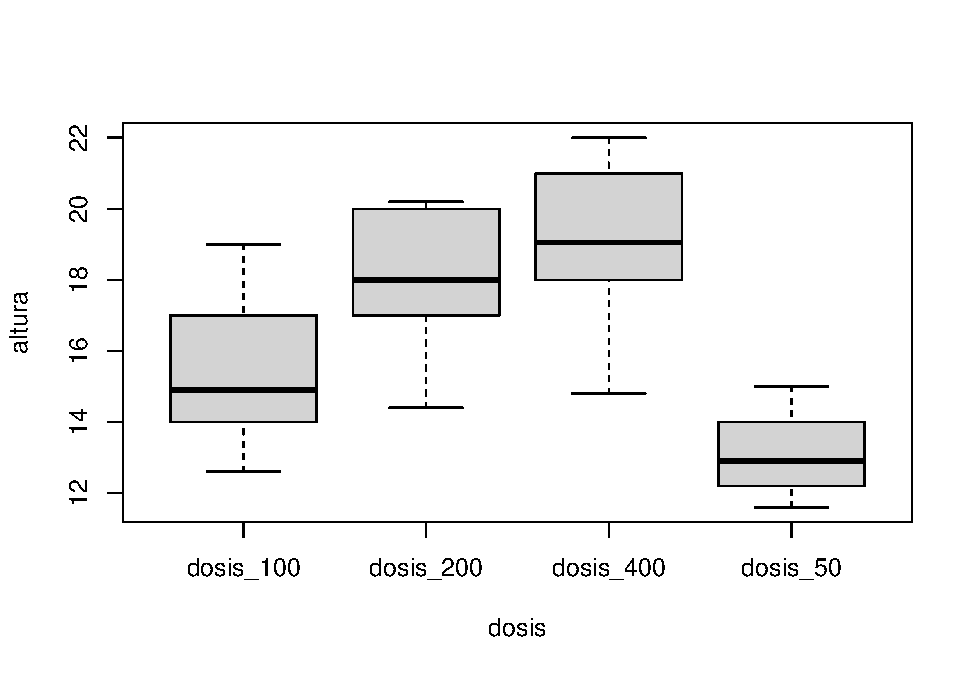
\includegraphics{_main_files/figure-latex/unnamed-chunk-73-1.pdf}

Para evaluar si las varianzas de los distintos grupos son homogéneas, podemos aplicar la prueba de homogeneidad de varianzas de Bartlett, con la siguiente hipótesis nula \(H_0\) e hipótesis alternativa \(H_1\):

\[ \begin{matrix}
H_0:\sigma_1^2=...=\sigma_k^2\\
H_1:\sigma_i^2 \neq \sigma_j^2, \,\, \forall i\neq j
\end{matrix}\]

Solicitamos a R que se aplique la prueba con la siguiente instrucción:

\begin{Shaded}
\begin{Highlighting}[]
\FunctionTok{bartlett.test}\NormalTok{(altura }\SpecialCharTok{\textasciitilde{}}\NormalTok{ dosis, }\AttributeTok{data =}\NormalTok{ rendimiento)}
\end{Highlighting}
\end{Shaded}

\begin{verbatim}
## 
##  Bartlett test of homogeneity of variances
## 
## data:  altura by dosis
## Bartlett's K-squared = 4.8838, df = 3, p-value = 0.1805
\end{verbatim}

Una vez verificado el supuesto de homogeneidad de varianzas, podemos solicitar el análisis de varianza en una clasificación de la siguiente manera:

\begin{Shaded}
\begin{Highlighting}[]
\NormalTok{aov.out }\OtherTok{\textless{}{-}} \FunctionTok{aov}\NormalTok{(altura }\SpecialCharTok{\textasciitilde{}}\NormalTok{ dosis, }\AttributeTok{data =}\NormalTok{ rendimiento)}
\FunctionTok{summary}\NormalTok{(aov.out)}
\end{Highlighting}
\end{Shaded}

\begin{verbatim}
##             Df Sum Sq Mean Sq F value   Pr(>F)    
## dosis        3  214.7   71.57   19.35 1.21e-07 ***
## Residuals   36  133.1    3.70                     
## ---
## Signif. codes:  0 '***' 0.001 '**' 0.01 '*' 0.05 '.' 0.1 ' ' 1
\end{verbatim}

Extraemos ahora los residuales y los analizamos de manera gráfica, verificando su normalidad:

\begin{Shaded}
\begin{Highlighting}[]
\NormalTok{aov\_residuals }\OtherTok{\textless{}{-}}\NormalTok{ aov.out}\SpecialCharTok{$}\NormalTok{residuals}
\FunctionTok{hist}\NormalTok{(aov\_residuals)}
\end{Highlighting}
\end{Shaded}

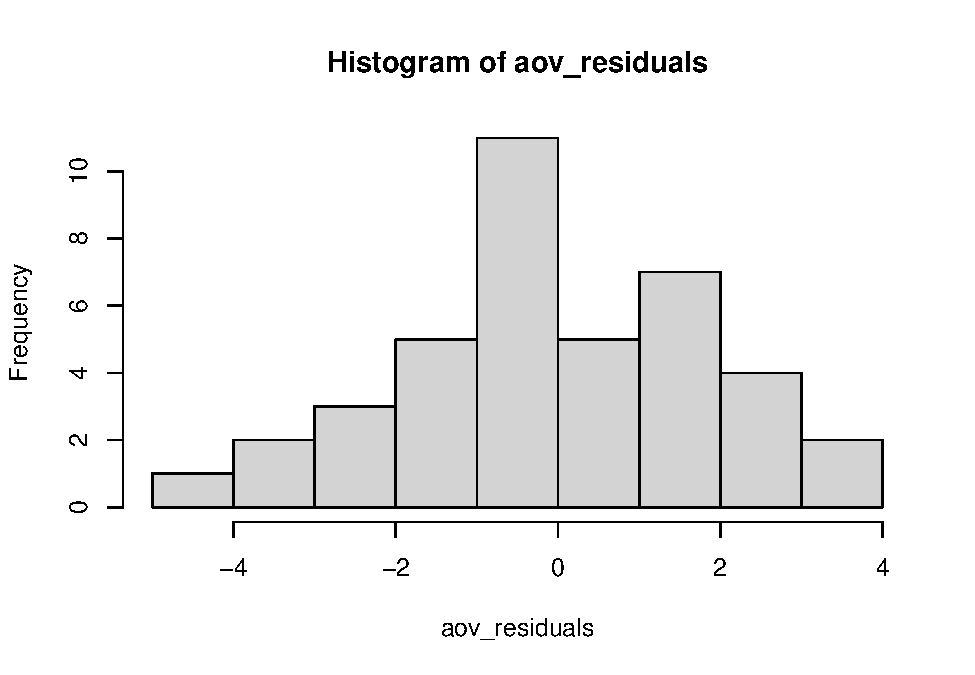
\includegraphics{_main_files/figure-latex/unnamed-chunk-76-1.pdf}

o utilizando una prueba cuantil-cuantil

\begin{Shaded}
\begin{Highlighting}[]
\FunctionTok{qqnorm}\NormalTok{(aov\_residuals)}
\FunctionTok{qqline}\NormalTok{(aov\_residuals,}\AttributeTok{col=}\DecValTok{2}\NormalTok{)}
\end{Highlighting}
\end{Shaded}

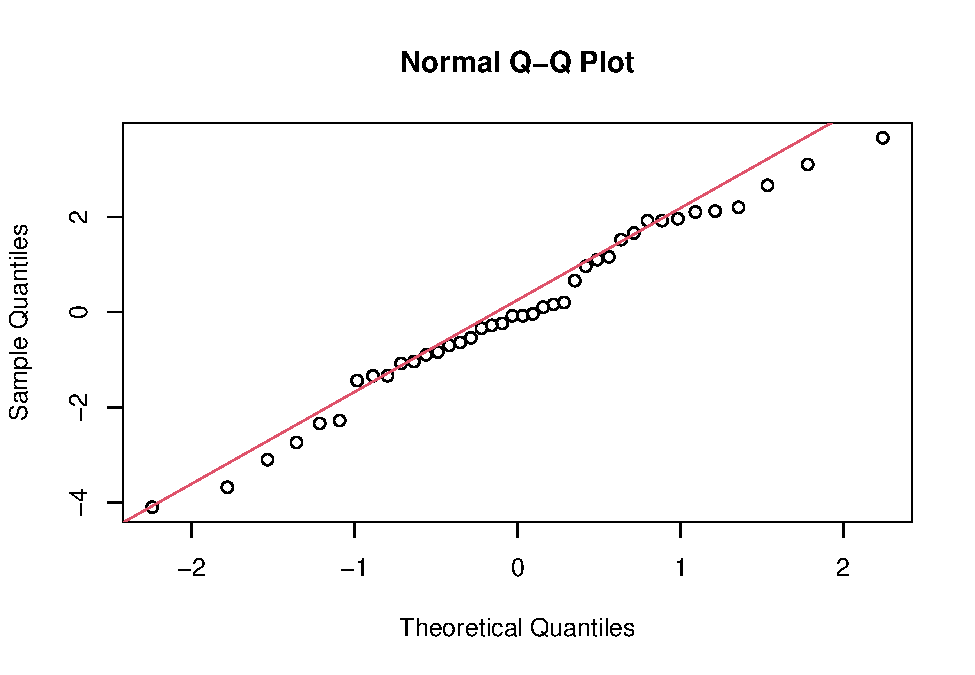
\includegraphics{_main_files/figure-latex/unnamed-chunk-77-1.pdf}

o más formalmente, podemos verificar la normalidad de residuales a través de una prueba de Shapiro-Wilk:

\begin{Shaded}
\begin{Highlighting}[]
\FunctionTok{shapiro.test}\NormalTok{(}\AttributeTok{x=}\NormalTok{aov\_residuals)}
\end{Highlighting}
\end{Shaded}

\begin{verbatim}
## 
##  Shapiro-Wilk normality test
## 
## data:  aov_residuals
## W = 0.98177, p-value = 0.7547
\end{verbatim}

Finalmente, podemos solicitar una prueba post Hoc, como la de Tukey, de la siguiente manera:

\begin{Shaded}
\begin{Highlighting}[]
\FunctionTok{TukeyHSD}\NormalTok{(aov.out, }\AttributeTok{conf.level =} \FloatTok{0.95}\NormalTok{)}
\end{Highlighting}
\end{Shaded}

\begin{verbatim}
##   Tukey multiple comparisons of means
##     95% family-wise confidence level
## 
## Fit: aov(formula = altura ~ dosis, data = rendimiento)
## 
## $dosis
##                      diff        lwr         upr     p adj
## dosis_200-dosis_100  2.74  0.4238594  5.05614056 0.0150760
## dosis_400-dosis_100  3.56  1.2438594  5.87614056 0.0011022
## dosis_50-dosis_100  -2.30 -4.6161406  0.01614056 0.0521923
## dosis_400-dosis_200  0.82 -1.4961406  3.13614056 0.7762839
## dosis_50-dosis_200  -5.04 -7.3561406 -2.72385944 0.0000062
## dosis_50-dosis_400  -5.86 -8.1761406 -3.54385944 0.0000003
\end{verbatim}

  \bibliography{book.bib,packages.bib}

\end{document}
